\documentclass[preprint,3p,11pt,authoryear]{elsarticle}

\usepackage{amsmath,amssymb,amsthm}

% Float placement. The two-row figures run to about 5.5 inches once scaled to
% the text width, and with their captions they exceed the default \topfraction
% of 0.7. LaTeX then defers them, and because floats cannot overtake one
% another, every later figure queues behind the first deferred one and the whole
% set lands at the end of the document. These fractions let a tall float take
% the page it needs near the text that refers to it.
\renewcommand{\topfraction}{0.92}
\renewcommand{\bottomfraction}{0.85}
\renewcommand{\textfraction}{0.07}
\renewcommand{\floatpagefraction}{0.72}
\setcounter{topnumber}{2}
\setcounter{bottomnumber}{2}
\setcounter{totalnumber}{3}
\usepackage{stmaryrd}  % \bigsqcap
\usepackage{booktabs}
\usepackage{graphicx}
\usepackage{xspace}
\usepackage{microtype}
\usepackage{url}
\usepackage[colorlinks=true,allcolors=blue]{hyperref}

\graphicspath{{../results/figures/}}
% Generated by tools/make_macros.py -- do not edit by hand.
% Every numeric result in the manuscript comes from this file.
\newcommand{\ABcases}{10\,000\xspace}
\newcommand{\Acases}{98\,385\xspace}
\newcommand{\Achecks}{787\,443\xspace}
\newcommand{\Acomp}{363\xspace}
\newcommand{\Afailed}{0\xspace}
\newcommand{\Amaxlen}{8\xspace}
\newcommand{\Awords}{9\,840\xspace}
\newcommand{\BOneFootprint}{0\xspace}
\newcommand{\BOneInterior}{10\,000\xspace}
\newcommand{\BThreeFootprint}{0\xspace}
\newcommand{\BThreeInterior}{0\xspace}
\newcommand{\BTwoFootprint}{10\,000\xspace}
\newcommand{\BTwoInterior}{0\xspace}
\newcommand{\BZeroFootprint}{10\,000\xspace}
\newcommand{\BZeroInterior}{10\,000\xspace}
\newcommand{\BbaseFive}{9\,455\xspace}
\newcommand{\BbaseLineageOne}{10\,000\xspace}
\newcommand{\BbaseOne}{9\,455\xspace}
\newcommand{\BbaseOnePct}{94.5\xspace}
\newcommand{\BbaseSupportOne}{0\xspace}
\newcommand{\BbaseUnverOne}{7\,222\xspace}
\newcommand{\BctrlDev}{0.0070\xspace}
\newcommand{\BctrlDevPct}{0.70\xspace}
\newcommand{\Bdepths}{5\xspace}
\newcommand{\BemAll}{0\xspace}
\newcommand{\BemLineage}{0\xspace}
\newcommand{\BemOpAll}{0\xspace}
\newcommand{\BemUnver}{0\xspace}
\newcommand{\Bintervals}{64\xspace}
\newcommand{\BopCount}{9\xspace}
\newcommand{\BopMax}{100.0\xspace}
\newcommand{\BopMin}{94.3\xspace}
\newcommand{\Btimelines}{10\,000\xspace}
\newcommand{\Cbase}{600\xspace}
\newcommand{\CbaseLineage}{600\xspace}
\newcommand{\Cclips}{600\xspace}
\newcommand{\CcorpusFs}{16\,000\xspace}
\newcommand{\CcorpusMismatch}{0\xspace}
\newcommand{\Cem}{0\xspace}
\newcommand{\CemLineage}{0\xspace}
\newcommand{\Cexact}{600\xspace}
\newcommand{\Cgen}{600\xspace}
\newcommand{\Dbase}{3\,600\xspace}
\newcommand{\DbaseLineage}{4\,200\xspace}
\newcommand{\Ddeterm}{0\xspace}
\newcommand{\DdetermN}{100\xspace}
\newcommand{\Dem}{0\xspace}
\newcommand{\DemLineage}{0\xspace}
\newcommand{\DguardOK}{all\xspace}
\newcommand{\DmaxDev}{681\xspace}
\newcommand{\DmeanEmIv}{3.13\xspace}
\newcommand{\DmpThreeDev}{31\xspace}
\newcommand{\DresampleDev}{0\xspace}
\newcommand{\Druns}{4\,800\xspace}
\newcommand{\DsilenceDev}{681\xspace}
\newcommand{\DstretchDev}{471\xspace}
\newcommand{\Dtransforms}{8\xspace}
\newcommand{\DzeroBase}{2\xspace}
\newcommand{\Eclips}{60\xspace}
\newcommand{\Econds}{5\xspace}
\newcommand{\Ederived}{60\xspace}
\newcommand{\Ereenc}{60\xspace}
\newcommand{\Estripped}{60\xspace}
\newcommand{\Etampered}{60\xspace}
\newcommand{\Evalid}{60\xspace}
\newcommand{\Eviol}{0\xspace}
\newcommand{\Fassertion}{120\xspace}
\newcommand{\Fclips}{40\xspace}
\newcommand{\Fcontainers}{3\xspace}
\newcommand{\Fderived}{120\xspace}
\newcommand{\Ffilechanged}{120\xspace}
\newcommand{\Fmismatch}{0\xspace}
\newcommand{\FmismatchPolicy}{0\xspace}
\newcommand{\Fparent}{120\xspace}
\newcommand{\Ftotal}{120\xspace}
\newcommand{\Ftrusted}{120\xspace}
\newcommand{\Fvalfail}{0\xspace}
\newcommand{\Gassertion}{1\,268\xspace}
\newcommand{\Gbase}{0.39\xspace}
\newcommand{\Gem}{0.81\xspace}
\newcommand{\GffmpegPct}{0.099\xspace}
\newcommand{\Gmanifest}{14\,854\xspace}
\newcommand{\GmaxIntervals}{256\xspace}
\newcommand{\GperInterval}{333\xspace}
\newcommand{\GperIntervalUs}{10.2\xspace}
\newcommand{\Gratio}{2.08\xspace}
\newcommand{\Greps}{30\xspace}
\newcommand{\Gsign}{13.2\xspace}
\newcommand{\GsignQa}{13.1\xspace}
\newcommand{\GsignQb}{13.4\xspace}
\newcommand{\Gval}{11.0\xspace}
\newcommand{\GvalQa}{10.9\xspace}
\newcommand{\GvalQb}{11.1\xspace}
\newcommand{\Hcases}{9\,804\xspace}
\newcommand{\Hdelta}{0\xspace}
\newcommand{\Hdis}{0\xspace}
\newcommand{\Rcommit}{d60a58e2edbe74b4bcacdbbb38228d8eddc4c05c\xspace}
\newcommand{\Rtag}{v1.0.0\xspace}
\newcommand{\Tfail}{0\xspace}
\newcommand{\Tpass}{27\xspace}
\newcommand{\Ttotal}{27\xspace}
\newcommand{\VcTwopatool}{0.27.2\xspace}
\newcommand{\Vespeak}{1.52.0\xspace}
\newcommand{\Vffmpeg}{9.0.1\xspace}
\newcommand{\Vnode}{v26.0.0\xspace}
\newcommand{\Vpython}{3.11.15\xspace}


\newtheorem{proposition}{Proposition}
\newtheorem{theorem}{Theorem}
\newcommand{\C}{\ensuremath{C}}
\newcommand{\G}{\ensuremath{G}}
\newcommand{\Dy}{\ensuremath{D_y}}
\journal{Forensic Science International: Digital Investigation}

% Reference-list spacing. The default leaves the last two entries alone on a
% page; this keeps them with the list without touching any entry.
\setlength{\bibsep}{0pt plus 0.1ex}
% Fourteen floats at the class defaults spend about a page on the white space
% around them alone. These are the class values less a few points each, which
% keeps floats clearly separated from the text without the excess space.
\setlength{\textfloatsep}{12pt plus 2pt minus 3pt}
\setlength{\intextsep}{10pt plus 2pt minus 3pt}
\setlength{\floatsep}{8pt plus 2pt minus 2pt}
\setlength{\abovecaptionskip}{5pt}
\setlength{\belowcaptionskip}{2pt}
% Line numbers for review; comment out \linenumbers for the camera-ready.
\usepackage{lineno}
\linenumbers

\begin{document}

\begin{frontmatter}

\title{Evidence-Monotone Audio Representation: Preventing Provenance
Promotion Across Derived Audio Transformations}

\author[aur]{Alejandro Urias\corref{cor}}
\ead{alex@aurtech.mx}
\cortext[cor]{Corresponding author. ORCID: 0009-0007-3147-323X.}
\address[aur]{Independent researcher, Hermosillo, Sonora, Mexico}

\begin{abstract}
Derived audio can keep its waveform while silently strengthening what it
says about its origin. Under a boundary-only inheritance policy, a constructed reference and not any
named product, a clip assembled from captured and generated material, then
trimmed, resampled and re-encoded, emerges described as captured-only. We specify an operator contract for derived audio:
over the complete required source set, provenance unions, same-channel support
minimises, applicability intersects and lineage unions, and an unverified source
interval is absorbing. The algebra is a known meet-semilattice
construction; new are the executable temporal instantiation over
sample-exact intervals with declared kernel footprints, a signed transport
inside C2PA temporal regions, and its evaluation. No
model is trained.
Across \Achecks{} contract checks, \Btimelines{} adversarial timelines,
\Cclips{} mixed-origin clips transformed by stock FFmpeg and \Hcases{}
differential-oracle cases, complete-source propagation produced \Afailed{}
failures and \Dem{} promotions, while boundary-only inheritance promoted in
\Dbase{} of \Druns{} stock-FFmpeg transformation runs. Decoded essence was identical before and after signing in \Ftotal{}
round-trips, at \Gratio{}$\times$ the bookkeeping baseline. An independent reproduction on
unrelated hardware and a different FFmpeg major version returned every
conformance, promotion and oracle outcome unchanged and found two
build-specific declarations its build does not satisfy,
reported as results rather than widened: the algebra holds by proof, the audio
instantiation only where its footprints were measured. The
contract constrains what a derived representation may claim about its sources,
and binds only an operator that implements it; it does not detect deepfakes,
and a valid signature proves only that an assertion was signed.
\end{abstract}

\begin{keyword}
digital evidence \sep media provenance \sep content credentials \sep C2PA \sep
audio forensics \sep derived media \sep reproducibility
\end{keyword}

\end{frontmatter}

\section{Introduction}
\label{sec:intro}

Speech can now be generated convincingly enough that ``is this recording
real?'' is answered less and less reliably by listening. Detection asks whether
a signal carries the traces of synthesis \citep{pham2025survey,wang2026asvspoof5};
provenance asks what an asset's own signed history says about where it came from
\citep{c2pa24}. This work is about the second question, so nothing here is a
detection result.

Provenance systems bind assertions to an asset. They do not, on their own, say
what a \emph{derived} asset is entitled to assert, and derivation is routine: a
clip is trimmed, spliced, resampled and re-encoded before it reaches an
examiner, and each step writes a new manifest. The C2PA specification names the
relationship of such an asset to its input \texttt{parentOf}
\citep[Table~10, \S18.16.3]{c2pa24}, and its vocabulary can carry everything the
problem needs: \texttt{componentOf} ingredients with their own histories, a
\texttt{digitalSourceType} for generative origin, assertions scoped to a
temporal range. What the text does not prescribe, and we searched it for such a
rule, is the \emph{reduction}: the aggregate evidence state a derived interval
should emit when the component histories it represents disagree. The
coalition's July 2026 guidance on identifying synthetic content develops the
vocabulary for declaring AI involvement and localising it to regions
\citep{c2pa2026synthetic}; that is guidance on how to \emph{represent} what
happened to part of an asset, and it is complementary to what this paper
supplies, the rule for what a derived interval may \emph{claim} once its parts
disagree.

Consider five consecutive source intervals of a
recording whose third is generated speech. A derived asset representing all five
can be described from its retained boundaries, which are captured, and emerge
labelled captured-only; the decoded audio is bit-identical either way
(Figure~\ref{fig:counterexample}). An examiner reading that claim is being told
something stronger than the sources support, by a chain in which no signature
was forged, and wherever a disclosure obligation is discharged by reading a
manifest rather than inspecting a signal the result is not a missed detection
but a confident wrong answer with a valid signature attached.

We call this \emph{provenance promotion}: a derived representation acquiring a
stronger evidential claim than the complete source material it represents,
without any change to the decoded signal. The requirement that prevents it,
\emph{evidence monotonicity}, is that along a chain of representation-only
transformations the emitted claim is no stronger than the meet of every required
source, ancestry accumulates rather than disappears, and the absence of verified
evidence is absorbing.

Digital forensics already treats the step from stored evidence to
software-derived representation as a place where meaning can change, and two
failure modes recur: what a representation aggregates away
\citep{hargreaves2024abstract,andersen2025toolbias}, and how far the same
nominal input is read differently by different builds and versions
\citep{nordvik2022exfat,kuelper2026testdriven}. Derived-media provenance meets
both at once: heterogeneous source evidence has to be reduced to one claim, and
the processing dependencies that decide which sources count are fixed by the
build, so a conservative reduction rule and validated dependency declarations
are both needed.

An earlier instantiation of that requirement exists for spatial data, where
derived terrain geometry can overstate the evidence of the source arc it
replaces \citep{urias2026emtrf}. This work asks whether the requirement is
usable in a temporal medium with a real signed transport and real processing
software, and what it costs. What is inherited and what is new, row by row, is
Supplementary Note~\NoteTransfer{}, and no earlier result is reused: the algebra transfers, and the temporal
interval maps, the kernel-footprint problem, the validations against
third-party processing, signal transparency and the signed transport have no
spatial analogue.


The algebra, a meet over
a semilattice of labels with union of ancestry and an absorbing bottom element,
is an instance of constructions that are decades old, in semiring-based
provenance annotation \citep{green2007provenance} and in label lattices for
secure information flow \citep{denning1976lattice,goguen1982noninterference}.
We do not claim the non-amplification property as a new theorem; we state it as
an instance, prove the one part specific to the temporal setting, and locate the
contribution in what is executable and measured.

\paragraph{Contributions} Each is traceable to a completed experiment.

\begin{enumerate}
\item \textbf{The contract, and its temporal instantiation.} An operator
  contract for derived media stated without reference to any modality, its
  non-amplification property presented as an instance of a known
  meet-semilattice construction (Section~\ref{sec:model}); instantiated over
  sample-exact half-open intervals for eight representation operators, each
  with a declared conservative kernel footprint, with a footprint-monotonicity
  result showing that over-approximating the required source set is always safe
  (Section~\ref{sec:audio}, Proposition~\ref{prop:footprint}).
\item \textbf{A signed transport, and what each part of the rule buys.}
  Interval evidence carried inside C2PA temporal regions of interest, surviving
  derivation and re-signing on \Fcontainers{} containers with \Ftotal{}
  round-trips, with a C2PA-native composition of signed captured and generated
  \texttt{componentOf} ingredients (Sections~\ref{sec:transport},
  \ref{sec:res-transport}, \ref{sec:res-composition}); and a policy ablation
  showing that complete-source aggregation and declared kernel footprints are
  each necessary and neither sufficient (Section~\ref{sec:res-ablation}).
\item \textbf{Evidence that it holds, and what it costs.} An executable
  conformance suite of \Achecks{} checks over every source word of length up to
  \Amaxlen{} over $\{\C,\G,\bot\}$ with \Afailed{} failures, and a two-language
  differential over \Hcases{} frozen cases with \Hdis{} disagreements, those
  frozen cases being the conformance target a third-party reimplementation can
  be run against (Sections~\ref{sec:res-conformance},
  \ref{sec:res-oracle}); \Cclips{} mixed-origin clips processed entirely by
  stock FFmpeg, with the interval mapping validated against software we do not
  control (Section~\ref{sec:res-corpus}) and the declared footprints tested
  separately by differential influence probes
  (Section~\ref{sec:res-containment}), since agreement on output length says
  nothing about how far a dependency reaches, both passes packaged as
  \path{tools/calibrate_footprint.py}; and cost on both axes, runtime, where
  bookkeeping is \GffmpegPct{}\% of the processing it accompanies and the
  assertion grows at \GperInterval{}~B per evidence interval
  (Section~\ref{sec:res-overhead}), and \emph{evidential}, a claim-dilution
  metric priced in samples per ancestry boundary rather than in fractions of
  the asset (Section~\ref{sec:res-dilution}).
\end{enumerate}

The contract does not infer authenticity from acoustic features; it prevents a
provenance-aware chain from promoting a mixed or unverified source interval
into a stronger captured-only class, and Section~\ref{sec:threat} states what
it does when evidence is absent. It is orthogonal to passive deepfake detectors
and to watermarking, and composes with either. Transparency obligations under
Article~50 of Regulation (EU) 2024/1689 became applicable on 2~August 2026
\citep{euaiact}, which makes machine-readable origin claims about derived media
operationally relevant; we make no legal claim about what any disclosure regime
requires.

\begin{figure}[htbp]
\centering
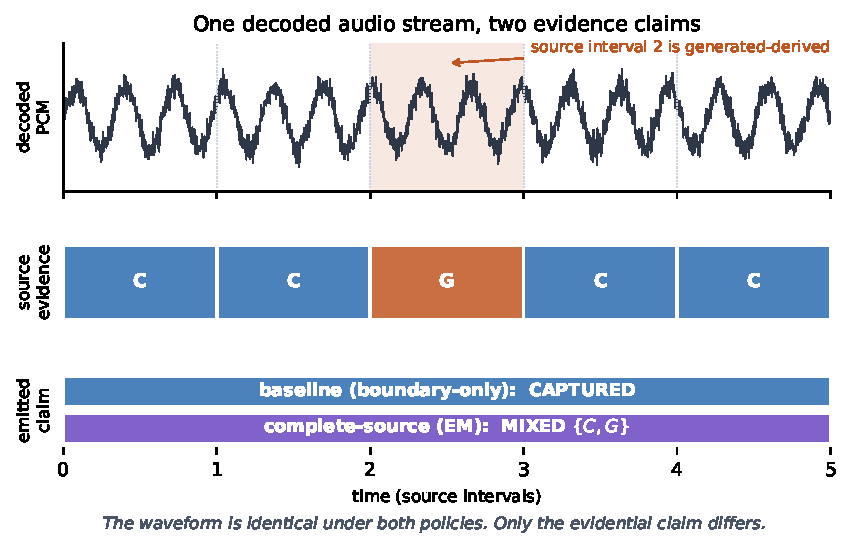
\includegraphics[width=\linewidth]{fig1_counterexample.pdf}
\caption{The minimal temporal counterexample. Five source intervals, of which
the third is generated-derived. A boundary-only reading of the retained region
sees captured evidence at both ends and may emit \textsc{captured}; the
complete-source rule sees $\C+\C+\G+\C+\C$ and emits \textsc{mixed}
$\{\C,\G\}$. The decoded audio is identical under both policies.}
\label{fig:counterexample}
\end{figure}

\section{Related work}
\label{sec:related}

\paragraph{Detection of synthetic speech} Anti-spoofing and deepfake-speech
detection classify a signal by its acoustic traces, and lose accuracy under
unseen attacks and codecs, as documented
\citep{wang2026asvspoof5,pham2025survey}. That line guarantees a decision about
a signal; it does not constrain what a derived asset may assert about its own
sources, and it needs no source evidence to exist.

\paragraph{Watermarking and soft bindings} Localised audio watermarking marks
generated speech at synthesis time and detects the mark per region
\citep{sanroman2024audioseal}; C2PA treats watermarks and fingerprints as
\emph{soft bindings} that recover a manifest separated from its asset
\citep[\S18.10]{c2pa24}. Neither defines the aggregate claim of a derived asset
whose sources differ, and a region carrying no mark is not thereby captured.

\paragraph{Cryptographic media provenance} C2PA binds signed assertions and
transformation history to an asset, defines the ingredient relationships
\texttt{parentOf}, \texttt{componentOf} and \texttt{inputTo}, and scopes
assertions to temporal regions of interest \citep[\S18.2.2.3,
\S18.16.3]{c2pa24}. Security analyses report problems in the cryptographic and
trust layers \citep{golaszewski2026c2pa}, and related work constructs assets
whose manifest and watermark contradict each other while each passes its own
verification \citep{nemecek2026contradictions}. Our concern is a different
layer, orthogonal to both: assuming keys are intact, signatures verify and no
assertion is omitted in bad faith, is the assertion a conforming derived asset
emits conservative with respect to every source interval it represents? The
specification preserves a great deal, since a \texttt{componentOf} ingredient
carries its own manifest and a generative component its
\texttt{digitalSourceType} \citep[\S18.16.3]{c2pa24}, and a consumer walking
the full graph could reconstruct everything. What version~2.4 does not define
is the aggregate: no normative rule states that a derived interval's own claim
must be the conservative reduction over all its components rather than an
inheritance from its parent. Our composition experiment is the evidence: every composition carries
two ingredients whose declared source types disagree, and the official
validator reports each as valid without computing or requiring any aggregate
over them (Section~\ref{sec:res-composition}).

\paragraph{Inferring audio provenance from the signal} \emph{Audio provenance
analysis} reconstructs content reuse and parent-child relations across a
heterogeneous collection with no prior knowledge of its contents, combining
partial matching with phylogeny \citep{gerhardt2024provenance}. That line
infers a lineage where none was recorded; the contract here assumes signed
source evidence exists and constrains how a known operator may aggregate it. A
pipeline could reasonably use the first to recover a lineage and the second to
decide what the recovered lineage entitles a derived interval to claim.

\paragraph{Provenance for edited audio} Chunk-localised speech provenance binds
short segments to an issuer-signed original through perceptual fingerprints and
Merkle commitments, addressing the fragility of hard bindings under re-encoding
\citep{ono2026merklespeech}; zero-knowledge constructions prove an edit was
drawn from an allowed set while hiding source, edits and device
\citep{fu2026trustvoice}. Neither states an aggregation rule for when the
represented sources disagree, and neither proves non-amplification.

\paragraph{Provenance models and information flow} W3C PROV records derivation
as a graph \citep{w3c2013prov}: a PROV graph for the five-interval
counterexample would hold \texttt{wasDerivedFrom} edges to all five sources, a
complete and true record, and still say nothing about which \emph{claim} the
derived segment may emit. The machinery for constraining that reading is
established: provenance semirings annotate derived data so that combination is
associative and distributes over alternative derivations
\citep{green2007provenance}, though idempotence, which the meet here has, is
not part of that framework and is incompatible with several of its instances;
information-flow lattices require combination to move only in the conservative
direction \citep{denning1976lattice,goguen1982noninterference}. The property we
need is the meet in such a structure, and we present it as such.

\paragraph{Forensic representation and tool-dependent interpretation}
\citet{hargreaves2024abstract} model a forensic tool as connected processing
stages in which an error introduced at one stage propagates downstream unless
intermediate outputs are exposed and validated, and empirical work fills in
what that costs. \citet{andersen2025toolbias} reported examiner errors
associated with misleading presentation in the semi-automated tools used in
that study, Cellebrite and APOLLO, naming aggregation, missing detail and
timestamp presentation among the contributing factors. Interpretation also
varies by implementation rather than by specification:
\citet{nordvik2022exfat} measured substantial inconsistencies in exFAT
timestamp handling across the operating systems and the four forensic tools
they examined, among them Autopsy and EnCase Examiner, and
\citet{kuelper2026testdriven} found largely undocumented changes in exported
report output across twenty-five versions of Autopsy. None of these
studies concerns provenance or demonstrates promotion, and the products named
in them appear here only as their subjects. The premise they establish is that
preserving source data is not sufficient if the derived representation changes
the evidential meaning an examiner sees.

\paragraph{What is missing} Table~\ref{tab:related} places these lines side by side.
No row provides an operator-level complete-source rule instantiated over media
time and carried in a signed transport; that combination is what this work
contributes, and the matrix behind the table, with search dates and query
strings, is Supplementary Note~\NoteNovelty{}.

\begin{table}[t]
\centering
\caption{Positioning. Each row names a guarantee the line already provides, then
the evidence property it does not, by itself, enforce on a derived audio
interval. The contribution here is the joint enforcement of the right-hand
column through representation-only operators, not the reinvention of any
left-hand guarantee.}
\label{tab:related}
\small
\begin{tabular}{p{0.27\linewidth}p{0.30\linewidth}p{0.33\linewidth}}
\toprule
Line of work & Established guarantee or finding & Left unenforced on a derived interval \\
\midrule
Synthetic-speech detection \citep{wang2026asvspoof5,pham2025survey} &
A decision about a signal from its acoustic traces &
What the derived asset may assert about its own sources \\
\addlinespace
Localised watermarking and soft bindings \citep{sanroman2024audioseal,c2pa24} &
Region-level presence of a mark; recovery of a separated manifest &
Aggregation of heterogeneous source evidence into one claim \\
\addlinespace
Cryptographic provenance \citep{c2pa24} &
Signed assertions, ingredient relationships, temporal regions of interest &
A rule requiring the derived claim to be conservative over all ingredients \\
\addlinespace
C2PA security analysis and cross-layer attacks
\citep{golaszewski2026c2pa,nemecek2026contradictions} &
Weaknesses in the trust, timestamp and validator layers; contradictions between
layers &
Behaviour of a chain in which every layer is intact and honest \\
\addlinespace
Audio provenance analysis \citep{gerhardt2024provenance} &
Reconstruction of reuse and parent-child relations from unknown signals, via
partial matching and phylogeny &
What a derived interval may claim once its recorded evidence disagrees \\
\addlinespace
Provenance for edited audio \citep{ono2026merklespeech,fu2026trustvoice} &
Chunk-to-original binding after transport; zero-knowledge edit correctness &
An aggregation rule when represented sources disagree \\
\addlinespace
Provenance graphs and lineage \citep{w3c2013prov} &
A truthful record of derivation &
Operator-level monotonicity as an executable contract \\
\addlinespace
Provenance semirings and information-flow lattices
\citep{green2007provenance,denning1976lattice} &
The algebra of conservative combination &
A temporal media instantiation with a signed transport \\
\addlinespace
Forensic tool representation and validation
\citep{hargreaves2024abstract,andersen2025toolbias,nordvik2022exfat,kuelper2026testdriven} &
Evidence that representation and output can vary across processing stages,
tools and versions &
A conservative operator-level rule for what a derived interval may claim about
heterogeneous source evidence \\
\addlinespace
Verifiable chain-of-custody ledgers \citep{burri2020custody} &
That a record of handling is complete and unaltered &
What a derived asset may claim about material it represents \\
\bottomrule
\end{tabular}
\end{table}

Source attribution from the signal, such as identifying a recording
microphone \citep{qamhan2023microphone}, infers origin from the audio, where
this work reads no audio at all. A contract is worth nothing unless its
implementation can be checked, which is why the conformance suite of
Section~\ref{sec:res-conformance} is written against the requirements rather
than against our code.

\section{Threat model}
\label{sec:threat}

\paragraph{In scope} Provenance promotion and laundering through
representation-only transformations, under four conditions: source evidence
exists; the processing system holds the source-to-output mapping; the operator
is expected to conform to the contract; and cryptographic primitives and signing
keys are intact.

\paragraph{Out of scope} Capture devices that lie about what they recorded;
compromised signing keys; dishonest certificate authorities; unsigned media of
unknown origin; speaker identity; the truthfulness of what is said; semantic
misinformation; waveform-artefact deepfake detection; watermark removal; and
full provenance stripping followed by construction of a fresh, dishonest trust
chain. Attacks on the cryptographic and trust layers are the subject of separate
analyses \citep{golaszewski2026c2pa} and are assumed away here precisely so that
the residual semantic question is isolated.

\paragraph{Required behaviour when evidence is absent or invalid} The state is
\textsc{unverified} or \textsc{invalid}. It is never automatically ``fake'' and
never automatically ``captured''. An asset can lose its manifest for entirely
benign reasons, and nothing in this work licenses reading a missing manifest as
evidence of intent.

\paragraph{Malicious signer} Cryptographic validity proves that an assertion
was signed, not that it is true; a signer willing to assert falsehoods can
produce a valid manifest containing them, and no propagation rule can prevent
that. The contract constrains conforming operators, not a dishonest issuer. A
threat-model matrix pairing attacker capability against contract behaviour is
Supplementary Note~\NoteThreat{}.

\section{Formal model}
\label{sec:model}

\subsection{Evidence records}

Let a source asset be partitioned into elements. Each element $x$ carries an
evidence record
\begin{equation}
e_x = (P_x, S_x, A_x, L_x),
\end{equation}
where $P_x$ is provenance, $S_x$ maps each semantically typed support channel
to a value in the lifted domain
\begin{equation}
\mathcal{S} = \{\bot_{\mu}\} \cup [0,1],
\qquad \bot_{\mu} \preceq s \ \text{ for every } s \in [0,1],
\label{eq:supportdomain}
\end{equation}
$A_x$ records the scope over which each channel is declared applicable, and
$L_x$ is lineage. A channel can be \emph{unavailable}, written $\bot_{\mu}$,
and must then count as weaker than any numeric value it could have carried,
otherwise ``no emitted channel value is greater'' would be silent about a
channel that disappears entirely; $\preceq$ on $\mathcal{S}$ is the usual order
on $[0,1]$ extended with $\bot_{\mu}$ as least element.

Provenance is a set of ancestry atoms drawn from $\{\C, \G\}$, for
captured-derived and generated-derived sources. Mixed ancestry is $\{\C,\G\}$
and is produced only by union; it is never a primitive. Nothing in the algebra
below depends on the size of this set: $\{\C,\G\}$ is the v1 instantiation,
and a deployment carrying finer atoms, per capture device or per generator,
inherits the propositions unchanged. The absence of verified evidence is a
distinct state $\bot$. It is not an atom, and it is never silently
mapped onto $\C$ or $\G$. The labels \textsc{captured}, \textsc{generated}, \textsc{mixed} and
\textsc{unverified} are renderings; the normative fields are $P$, $S$, $A$
and $L$, and \textsc{real} is not a state anywhere in the model, the
implementation or the serialisation.

\subsection{The claim order and its meet}

Write $\widehat{\mathcal{C}} = \{\bot\} \cup (2^{\{\C,\G\}} \setminus
\emptyset)$ for the set of provenance claims, ordered by
\begin{equation}
q_1 \sqsubseteq q_2 \iff q_1 = \bot \ \text{ or }\ (q_2 \neq \bot \ \text{and}\
q_1 \supseteq q_2),
\label{eq:order}
\end{equation}
read ``$q_1$ is no stronger than $q_2$'': a larger atom set is a weaker
claim and $\bot$, which asserts nothing, is the bottom element. This is a
partial order under which two claims always have a greatest lower bound but
need not have an upper bound ($\{\C\}$ and $\{\G\}$ have none), so the
structure is a meet-semilattice rather than a lattice, with meet
\begin{equation}
q_1 \sqcap q_2 =
\begin{cases}
\bot & \text{if } q_1 = \bot \text{ or } q_2 = \bot,\\
q_1 \cup q_2 & \text{otherwise.}
\end{cases}
\label{eq:meet}
\end{equation}

This is a standard construction, an idempotent, commutative, associative
combination with an absorbing element, as in provenance semirings
\citep{green2007provenance} and information-flow lattices
\citep{denning1976lattice}; we record it rather than derive it.

\subsection{The complete-source operator}

Let a representation operator $T$ produce output element $y$ from the
\emph{complete required source set} $\Dy = \{x_1, \dots, x_k\}$. Two notions of
dependency diverge for some operators. The \emph{representational} dependency
of $y$ is the source content $y$ stands for; the \emph{computational}
dependency is the set of source samples that numerically influence its value.
The contract governs the representational reading, and the kernel footprint
reconciles the two where signal processing makes them bleed together: a
resampling filter makes neighbouring content influence $y$, and since that
influence cannot be distinguished from representation at the contract's level
of abstraction, the footprint conservatively enlarges $\Dy$ to cover it. The
one v1 operator for which the two readings diverge completely is amplitude
normalisation (Section~\ref{sec:limits}). Write
$\Dy^{\mu} = \{x \in \Dy : \mu \in A_x\}$ for the sources that declare channel
$\mu$ applicable. The contract requires:

\begin{description}
\item[(i) Provenance] $P_y = \bigsqcap_{x \in \Dy} P_x$, that is, the exact
  union of the required source provenance sets, with $\bot$ absorbing and with
  no invented ancestry.
\item[(ii) Support] if $P_y \neq \bot$, $\Dy^{\mu} \neq \emptyset$,
  $A_y(\mu) \neq \emptyset$ and every member of $\Dy^{\mu}$ supplies a value,
  then $S_y(\mu) = \min_{x \in \Dy^{\mu}} S_x(\mu)$; otherwise the channel is
  \emph{unavailable}; without the applicability condition a channel narrowed
to an empty scope under~(iii) would carry a number applicable nowhere.
  Requirement~(iv) strengthens the condition $\Dy^{\mu} \neq \emptyset$
  stated here to $\Dy^{\mu} = \Dy$.
\item[(iii) Applicability] the \emph{canonical} scope is
  $A_y(\mu) = \bigcap_{x \in \Dy^{\mu}} A_x(\mu)$, and an empty intersection
  makes the channel unavailable. A \emph{conforming} operator may emit any
  $A_y'(\mu) \subseteq A_y(\mu)$, never a broader one; conformance is the
  containment, the equality names the canonical reduction the reference
  implementation emits, and statements quantifying over conforming operators,
  Theorem~\ref{thm:composition} in particular, are read in that sense.
\item[(iv) No partial subsets] a channel is available on the output only if
  every required source declares it applicable \emph{and} supplies a value:
  $\Dy^{\mu} = \Dy$ is required, not merely $\Dy^{\mu} \neq \emptyset$. A
  channel unreported by some required source, or not applicable to it at all,
  is unavailable and is not computed from the remaining sources. The second
  half is what makes Proposition~\ref{prop:footprint} hold for channels:
  without it, enlarging $\Dy$ by a source that declares an otherwise
  inapplicable channel would raise that channel from unavailable to a value.
\item[(iv$'$) Unverified absorption for channels] if any required source is in
  state $\bot$, every numeric channel on the output is unavailable.
\item[(v) Lineage] $L_y = \bigcup_{x \in \Dy} L_x$, identifying the complete
  required source set. The record is carried per evidence-homogeneous interval,
  so $L_y$ names the assets required by \emph{that} interval and the interval's
  own bounds carry the placement.
\end{description}

Requirements~(iv) and~(iv$'$) are where this model is strictly stronger than
its spatial predecessor. (iv) costs expressiveness: sources with
different channel schemas yield no channel on a shared interval. (iv$'$) is
its companion for $\bot$, since computing a channel from the remaining
verified sources would be the partial-subset computation (iv) forbids. Both
are tested separately.

\subsection{Properties}

The guarantee below is that a derived claim can only lose.

\begin{proposition}[Non-promotion]
\label{prop:union}
Under~(i)--(iv$'$): $P_y \sqsubseteq P_x$ for every $x \in \Dy$, and no atom
appears in $P_y$ that appears in no required source; if any required source
has $P_x = \bot$ then $P_y = \bot$ and no numeric channel is emitted; and for
every channel $\mu$, $S_y(\mu) \preceq S_x(\mu)$ for every $x \in \Dy^{\mu}$
while $A_y(\mu)$ is no broader than any $A_x(\mu)$.
\end{proposition}
\begin{proof}
By~\eqref{eq:meet}, $P_y$ is $\bot$ if any source is, and $\bot \sqsubseteq q$
for every $q$; otherwise it is the union of the source sets, which contains
each $P_x$ and is therefore $\sqsubseteq P_x$ by~\eqref{eq:order}, and
membership of an atom in $P_y$ requires membership in some $P_x$.
Requirement~(iv$'$) withholds every channel when $P_y = \bot$. A minimum over
a set is bounded above by each member, (ii) refuses to emit unless every
applicable source supplies a value, and repeated intersection in~(iii) cannot
enlarge a set.
\end{proof}

\begin{theorem}[Closure under composition]
\label{thm:composition}
A finite composition of operators each satisfying~(i)--(v), including~(iv$'$),
satisfies the same requirements, and the composed claim is no stronger than the
meet over the union of all ancestral required source sets.
\end{theorem}
\begin{proof}
Associativity and commutativity of $\sqcap$ make the composed provenance the
meet over the union of the ancestral sets, so no ancestor is dropped or
invented; absorption of $\bot$ is preserved inductively because no later
operator receives a verified element in place of an unverified ancestor. For a
channel $\mu$, each operator either refuses the channel or emits a value bounded
by its applicable inputs, and transitivity of $\preceq$ bounds the final value by
every applicable ancestor. Repeated intersection cannot broaden a scope, and
lineage composes by union of the per-operator source maps.
\end{proof}

Theorem~\ref{thm:composition} is the standard consequence of combining in a
meet-semilattice; the next proposition is specific to the temporal setting and
is what makes the contract implementable against real processing software: more
possible source dependencies may weaken an output claim and can never
strengthen it, so erring towards a larger footprint errs safely.

\begin{proposition}[Footprint monotonicity]
\label{prop:footprint}
If $\Dy \subseteq \Dy'$ then the claim computed from $\Dy'$ is no stronger than
the claim computed from $\Dy$, and for every channel $\mu$ the value computed
from $\Dy'$ is $\preceq$ the value computed from $\Dy$ in $\mathcal{S}$.
\end{proposition}
\begin{proof}
Enlarging the index set of a union can only add atoms, and by~\eqref{eq:order}
a superset is a weaker claim; adding a source in state $\bot$ sends the claim to
$\bot$, which is weaker still.

For channels the argument runs through~(iv), which requires
$\Dy^{\mu} = \Dy$ for availability. Suppose $\mu$ is available on $\Dy'$. Then
every member of $\Dy'$ declares $\mu$ applicable and supplies a value, so every
member of $\Dy \subseteq \Dy'$ does too, and $\mu$ is available on $\Dy$ as
well; the emitted value is a minimum over the larger set $\Dy'$, which is no
larger than the minimum over $\Dy$. Suppose instead $\mu$ is unavailable on
$\Dy$. Some member of $\Dy$ then fails to declare $\mu$ applicable, fails to
supply a value, or is in state $\bot$; that same member lies in $\Dy'$, so $\mu$
is unavailable on $\Dy'$ as well, and $\bot_{\mu} \preceq \bot_{\mu}$. The
remaining case is an added source whose scope empties the intersection
in~(iii): requirements~(ii) and~(iii) then withhold the channel, giving
$\bot_{\mu}$, which by~\eqref{eq:supportdomain} is $\preceq$ every element of
$[0,1]$. Every case therefore moves down $\mathcal{S}$.

The condition $\Dy^{\mu} = \Dy$ carries the weight here. Under the weaker
$\Dy^{\mu} \neq \emptyset$ the statement is false: with $\Dy = \{x_1\}$ and
$\mu$ not applicable to $x_1$, enlarging to $\Dy' = \{x_1, x_2\}$ where $x_2$
declares $\mu$ with value $v$ would raise the channel from $\bot_{\mu}$ to $v$.
\end{proof}

Proposition~\ref{prop:footprint} is the practical result of this section: an
implementation does not need the exact dependency set of a filtered operator,
because a \emph{conservative over-approximation} is always safe and only
under-approximation can promote. That converts knowing which input samples
every output sample depends on inside a third-party codec into a tractable
requirement: declare a bound, and test that it holds.

\paragraph{Signal transparency (P8)} The contract must not change the audio.
The canonical essence of an asset is the SHA-256 of its decoded stream rendered
to signed 16-bit little-endian PCM at the asset's own rate and channel count,
and it must be identical whether the EM assertion or the baseline assertion is
attached. Whole-file hashes are unusable here because embedding a manifest
changes the file by construction (Section~\ref{sec:res-transport}).

\section{Audio instantiation}
\label{sec:audio}

\subsection{Temporal intervals}

All positions are sample indices on a named asset and all intervals are
half-open $[a,b)$, matching the C2PA convention that ``All start times are
inclusive of that moment in time, and all end times are, by default, exclusive
of it'' \citep[\S18.2.2.3]{c2pa24}. A source timeline is a gapless ordered
partition of an asset into evidence-homogeneous intervals.

\paragraph{The v1 support channel} Version~1 carries one typed channel,
\texttt{capture-support}, applicable over the single scope
\texttt{digital-asset}: the degree to which an interval's own record supports a
capture claim, on $\mathcal{S}$. It is not a detector output and is not
calibrated against any acoustic measurement: what this instantiation
demonstrates is that a typed channel aggregates by minimum, absorbs, intersects
its scope and survives the transport, not that its numbers carry forensic
meaning. The corpus and transport experiments assign \CaptSupport{} to
captured-derived and \GenSupport{} to generated-derived intervals, so a mixed
interval aggregates to \GenSupport{}; the enumeration sweeps a grid of values,
and the universal statement over $[0,1]$ comes from the proof. One scope cannot
exhibit disjoint or overlapping scopes, nor a channel applicable to one source
and not another, the case Proposition~\ref{prop:footprint} turns on; a
synthetic battery over \LscopeScopes{} scopes covers those
(Section~\ref{sec:res-conformance}).

An operator emits a set of \emph{map pieces} (Figure~\ref{fig:architecture}): output range $[o_a, o_b)$
represents source range $[s_a, s_b)$ on a named asset, with a footprint radius
in source samples. Where pieces overlap, as in a mix, the required source set of
an output interval is the union over every covering piece. The emitted output
partition is the pull-back of every source evidence boundary across every piece,
which gives each emitted interval a stable complete required source set.

\begin{figure}[tbp]
\centering
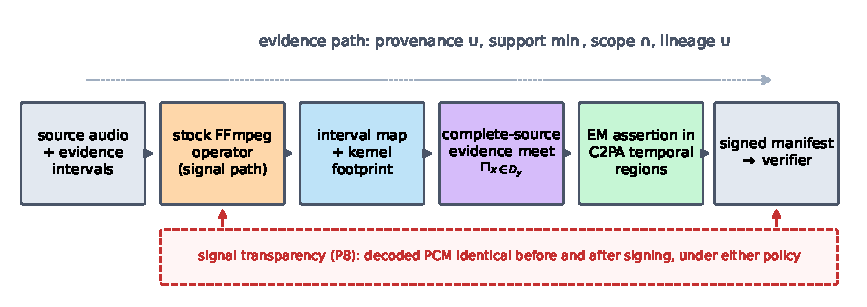
\includegraphics[width=\linewidth]{fig2_architecture.pdf}
\caption{Where the contract sits. Stock FFmpeg performs the transformation; the
interval map with its declared kernel footprint determines the complete required
source set; the complete-source meet produces the emitted evidence; the result
is serialised as C2PA temporal regions of interest and signed. The evidence path
never touches the signal path, which is what signal transparency (P8) measures.}
\label{fig:architecture}
\end{figure}

\subsection{The v1 operator set and its kernel footprints}

Table~\ref{tab:operators} gives the eight operators in scope with their mapping
and declared footprint. Pitch shifting is not a further primitive: it composes a rate change with a
compensating stretch, so Theorem~\ref{thm:composition} covers it and a named
regression test exercises the composite. Denoising, separation and enhancement are out of scope for v1
because their dependency structure needs modelling of its own; generative
editing differs more basically, since it may introduce new ancestry.

For a polyphase resampler the radius
follows from the pinned filter length and rate ratio. At \CcorpusFs{}~Hz \texttt{libmp3lame} emits
MPEG-2 LSF frames of \MpThreeGuard{} samples; the radius takes the larger
MPEG-1 long window, \MpThreeWindow{}, plus the encoder delay, giving
\MpThreeKernel{}, and one frame of alignment guard. That derivation is necessary but not sufficient: the pinned
\texttt{libmp3lame} runs with its bit reservoir enabled, which carries bits
across frames, so the encoder is stateful in a way no window-and-delay
argument captures. The declared \MpThreeDeclared{} is therefore an
\emph{empirically validated bound for this frozen configuration}, confirmed by
the probes of Section~\ref{sec:res-containment} at a measured reach of
\KmpThreeReach{}; a different bitrate, encoder or reservoir setting requires
re-probing. For overlap-add time stretching the footprint covers the analysis window
scaled by the tempo factor; for a frame-granular selector it covers the
difference between the exact retained-sample model and the implementation's
frame-aligned cuts. Two experiments check these numbers against software we do not control, and
they bound different quantities: Section~\ref{sec:res-corpus} measures
temporal mapping deviation, which informs the margin, and
Section~\ref{sec:res-containment} tests whether the \emph{declared}
footprint contains the measured source influence. For two operators the
measured reach exceeds the analytical support and is contained only by the
declaration as a whole, which is why the declaration, not either component, is
what an implementation uses. An implementation on a build for which the two quantities have not been
validated has no
declaration to use, and the contract leaves three courses: refuse the
operation, mark the interval unverified, which Section~\ref{sec:model} makes absorbing, or widen to
whole-asset dependency and pay the dilution of
Section~\ref{sec:res-dilution}. Emitting the claim an unvalidated
declaration would license is the one course forbidden.

\begin{table}[t]
\centering
\caption{The v1 operator set. The analytical column is a support radius derived
from the pinned algorithm configuration; the margin covers implementation
behaviour that the analysis does not capture, such as frame-granular cut points
and a correlation search range; the declared footprint is their sum and is the
quantity Section~\ref{sec:res-containment} probes.
All values are in
source samples for the configurations used in the experiments, so
transcoding takes a row per codec and the eight operators occupy nine rows;
concatenation assembles the corpus clips rather than transforming them
(Section~\ref{sec:corpus}), leaving the eight transformations
Section~\ref{sec:results} counts and, among those, the \Kops{} single-source
configurations Section~\ref{sec:res-containment} probes. By
Proposition~\ref{prop:footprint} erring large only weakens the emitted claim;
erring small is a conformance failure. These
values hold for one FFmpeg build and are not portable: on the build used in the independent reproduction of
Section~\ref{sec:res-independent}, the MP3 row is under-declared. Section~\ref{sec:limits} states the normalisation row's
representational reading and its tested alternative.}
\label{tab:operators}
\small
\begin{tabular}{p{0.24\linewidth}p{0.24\linewidth}rp{0.27\linewidth}}
\toprule
Operator & Source mapping & Footprint & Reason \\
\midrule
trim / crop & 1:1 on the retained range & 0 & exact \\
concatenate & 1:1 per part & 0 & exact \\
resample & $n_\mathrm{out}\!\cdot\!f_\mathrm{in}/f_\mathrm{out}$ & 33 & polyphase FIR \\
transcode (MP3) & 1:1 & 2304 & MDCT window + encoder delay \\
transcode (FLAC) & 1:1 & 0 & lossless \\
amplitude normalisation & 1:1 & 0 (strict: whole signal) & scalar gain \\
time stretch & $t_\mathrm{src}=\tau\,t_\mathrm{out}$ & 2577 & overlap-add window \\
silence removal & explicit retained runs & 2048 & frame-granular selector \\
mix / overlay & 1:1 from every covering source & 0 & sample-wise sum \\
\bottomrule
\end{tabular}

\end{table}

\subsection{The baseline reference policy}
\label{sec:baseline}

The comparison policy throughout is \emph{boundary-only, primary-parent
inheritance}: the derived output inherits from its parent ingredient, evaluated
at the first and last source elements of the retained region, ignoring kernel
footprints. It is a \textbf{constructed reference policy}, not a description
of any shipping product, and no claim is made here about what any named tool
does. Its motivation is the specification text: a derived asset's relationship
to its input is \texttt{parentOf}, ``a derived asset or asset rendition of this
ingredient'' \citep[Table~10, \S18.16.3]{c2pa24}, and the minimal way to
inherit from a parent over a retained region is to read its endpoints. Since
the specification does not define the reduction, every implementation that
derives an asset supplies one, deliberately or by default, and endpoint
inheritance is the reading its own vocabulary most directly suggests. The
baseline isolates one consequence of that underspecification without
attributing it to any implementation; how deployed software behaves would need
a survey this paper does not contain.

The baseline combines two independent shortcuts, boundary-only inheritance and
blindness to the kernel footprint, so the experiments also evaluate the two
intermediate policies that remove one shortcut each
(Section~\ref{sec:res-ablation}). That ablation keeps the comparison from
resting on the choice of baseline: a reader who disputes the composite policy
can read the result off the intermediate arm.

\subsection{Signed transport}
\label{sec:transport}

Evidence is carried as a namespaced C2PA assertion,
\texttt{\Clabel{}}, with one entry per output evidence
interval. Each entry gives a temporal region of interest as an \texttt{npt}
range \citep[\S18.2.2.3]{c2pa24}, the sample-exact bounds alongside it because
\texttt{npt} strings are lossy at sample resolution, the provenance atom list
(\texttt{null} for unverified, never an atom), the available support channels,
their applicability scopes, and the lineage set. Derivation records the source
as an ingredient with relationship \texttt{parentOf}; the specification requires
a corresponding \texttt{c2pa.opened} action carrying a hashed-URI reference to
that ingredient assertion \citep[\S15.11.3.2]{c2pa24}, which the claim generator
inserts. Composition records each source as a \texttt{componentOf} ingredient
carrying its full source manifest, with a \texttt{c2pa.placed} action
referencing each component's ingredient assertion \citep[\S18.16.3]{c2pa24},
so the transport exercises exactly the composition vocabulary whose missing
aggregation rule motivates the paper (Section~\ref{sec:res-composition}). The
full schema, with a worked manifest, is Supplementary Note~\NoteSchema{}.

The transport is a bridge, not a re-implementation: signing and validation are
performed by the official \texttt{c2patool}, so the transport guarantees are
the tool's. The choice of C2PA is not load-bearing; the same assertion can be
carried in a detached signed sidecar, and C2PA is used because it is the
deployed standard and tests the mapping against a real validator.

\section{Methods}
\label{sec:methods}

\subsection{Study design}

The experiments separate three questions that are easy to conflate: whether the
implementation realises the stated guarantees (a mathematical question, answered
by exhaustive enumeration and by differential testing); whether a competing
metadata rule produces counterexamples on adversarial and on realistic input (a
mechanism question, answered by frozen fixtures and a labelled corpus); and what
the contract costs (an engineering question, answered by timed repetitions).
Exact algebraic properties and finite-state classifications are reported as
deterministic counts and are not assigned $p$-values, and
Table~\ref{tab:boundary} states, for each class of claim, which evidence is
used for it and what that evidence does not establish. Fixture failure
frequencies characterise the frozen fixture family and are a \textbf{mechanism
stress rate}: they are not, and must not be read as, an estimate of how often
any deployed system promotes provenance.

\subsection{Deterministic fixtures}

Experiment~A enumerates every source word of length $1$ to \Amaxlen{} over
$\{\C, \G, \bot\}$, giving \Awords{} words, and pushes each through up to ten
operator configurations. Two configurations require a minimum word length: the inner trim needs at least three elements and silence removal at least two. So the \AwordsShortOne{} single-element words receive eight configurations,
the \AwordsShortTwo{} two-element words nine, and the remaining \AwordsFull{}
words the full ten, giving \Acases{} cases. Each case is checked against the property suite and against a closed-form
oracle that recomputes the expected state from the operator's nominal source
ranges without the evidence algebra; zero-footprint operators must match it
exactly, and kernel operators may only be weaker.

Experiment~B freezes \Btimelines{} timelines of \Bintervals{} source intervals
each, generated from a fixed seed, in which the majority of intervals are
captured and one to four \emph{non-boundary} intervals are replaced by generated
or unverified evidence. Each is pushed through composition chains of depth $1$
to \Bdepths{} and, separately, through each operator alone. Because the
anomalies are deliberately placed away from the boundaries, the baseline's
failure rate on this family is high by construction. To make that explicit,
the experiment includes a control arm in which anomaly positions are drawn uniformly
over all positions, for which the baseline's promotion probability has the
closed form $\binom{n-2}{k}/\binom{n}{k}$ for $k$ anomalies of a single type
over $n$ positions.

\subsection{Mixed-origin audio corpus}
\label{sec:corpus}

\Cclips{} clips are built deterministically, each of the form captured $\vert$
generated $\vert$ captured with sample-exact ground truth. Captured segments are
crops of LibriSpeech \texttt{dev-clean} \citep{panayotov2015librispeech},
CC~BY~4.0; generated segments are produced locally by eSpeak~NG formant
synthesis from phrases written for this study. No speaker is identified and no
voice is cloned. Segment durations are matched so that the generated region is
a modest interior interval. 

Because the evidence algebra reads no acoustic feature, the result cannot in
principle depend on signal character. A robustness arm demonstrates that
rather than leaving it to argument, rebuilding \CtwoNeuralN{} clips with a neural TTS
(Piper, a VITS-architecture engine with a voice trained on the public-domain
LJSpeech corpus) and overlaying \CtwoNoiseN{} clips with locally generated pink
noise at $-18$~dB so that every ancestry boundary is acoustically buried.

Concatenation and every subsequent transformation are performed by
\textbf{stock FFmpeg through its command line, with no project code in the
signal path}: the artefact that does or does not exhibit promotion is produced
by software the author does not control, and only the evidence policies are
under study.

\subsection{Metrics}

We report promotion counts and rates, lineage omissions, unverified-to-verified
promotions, support promotions, conformance failures, decoded-essence
mismatches, manifest validation outcomes, model-versus-implementation sample
deviations, runtime and metadata size. We deliberately do not report accuracy,
precision, recall, $F_1$ or AUC: no classifier is evaluated. Timing is
reported as medians with interquartile ranges over \Greps{} repetitions on a
single machine, an \Vcpu{} with \Vcores{} logical cores and \Vram{}~GiB,
running \Vos{}, Python~\Vpython{}, FFmpeg~\Vffmpeg{} and
\texttt{c2patool}~\VcTwopatool{}; every version is recorded in
\texttt{results/PREFLIGHT.txt}, regenerated on each run. Each repetition processes \Gclips{} clips in one process with no affinity or
power control and no warm-up, which moves the median by \GfirstIterPct{}\%.

\subsection{Reproducibility and AI use}

Every number in this manuscript is emitted by code into
\texttt{results/machine\_readable/}, converted into a LaTeX macro by a
generator script, and used in the text through that macro; no result is typed by
hand. Every figure is rendered from the same files. \texttt{run\_all.sh} exits
non-zero if any conformance check fails. Generative-AI tools were used as
programming and review assistants, under the declaration at the end of this
paper.

\section{Results}
\label{sec:results}

\subsection{Exhaustive conformance}
\label{sec:res-conformance}

Over \Awords{} source words and \Acases{} operator cases, the property suite
and the closed-form oracle together evaluated \Achecks{} checks with
\Afailed{} failures, including \Acomp{} explicit composition cases. Every named regression test passes, across the contract and review-regression
suites together: \Tpass{} of \Ttotal{}, with \Tfail{} failures
(Table~\ref{tab:main}).

That enumeration carries one channel over one scope, which is what the audio
instantiation uses, so it cannot reach the applicability cases of~(iii). A
separate synthetic battery covers those: over \LscopeScopes{} scopes, chosen so
that pairs are disjoint, nested and partially overlapping, it enumerates
\LscopeCases{} source-set enlargements and checks each against
Proposition~\ref{prop:footprint}, with \LscopeViolations{} violations.

An earlier version of requirement~(iv) withheld a
channel only when a required source declared it applicable and reported no
value, leaving a source to which the channel was not applicable at all to be
silently skipped. Under that rule the enumeration still passed all \Achecks{}
checks, because in v1 every non-$\bot$ source declares the one channel; the
battery fails it in \LscopeFailBad{} of \LscopeCases{} cases, each an
enlargement that raised a channel from unavailable to a value. The
monotonicity check had the same blind spot, comparing a channel only when it
was present on both sides. Both are fixed and the battery runs in the pipeline.

During development the suite failed on the overlay operator,
where the implementation evaluated overlapping map pieces independently and
emitted a captured claim and a generated claim over the same output interval
instead of one mixed claim; that was a defect in our own code, fixed by making the
output partition global across pieces. A conformance suite that has never
failed is evidence of nothing.

\subsection{Adversarial timelines}
\label{sec:res-adversarial}

On \Btimelines{} frozen timelines, boundary-only inheritance promoted the
provenance claim on \BbaseOne{} timelines (\BbaseOnePct{}\%) at composition
depth~1 and on \BbaseFive{} at depth~\Bdepths{}; complete-source propagation
produced \BemAll{} promotions summed over every depth, \BemUnver{}
unverified-to-verified promotions, \BemLineage{} lineage omissions and no
support promotion. Boundary-only inheritance omitted required lineage on
\BbaseLineageOne{} timelines at depth~1 and reported \BbaseUnverOne{}
unverified spans as verified.

The rate does not rise with depth, and that is the finding: the loss is
established at the first derivation and is irreversible, because once the
interior evidence is discarded no downstream operator can recover it
(Figure~\ref{fig:promotion}A). Across the \BopCount{} operator configurations
applied singly, baseline promotion ranged from \BopMin{}\% to \BopMax{}\% and
complete-source propagation produced \BemOpAll{} promotions
(Figure~\ref{fig:promotion}B). In the control arm, with anomaly positions
uniform over all positions, measured baseline rates agreed with the closed-form
prediction to within \BctrlDev{} in absolute rate (\BctrlDevPct{} percentage
points) in every cell (Figure~\ref{fig:promotion}C). The adversarial arm's near-unity rate is thus a property of the
construction, arithmetically predictable, and carries no information about
deployed software; the informative quantity is the exact zero on the other
side.

\begin{figure}[tbp]
\centering
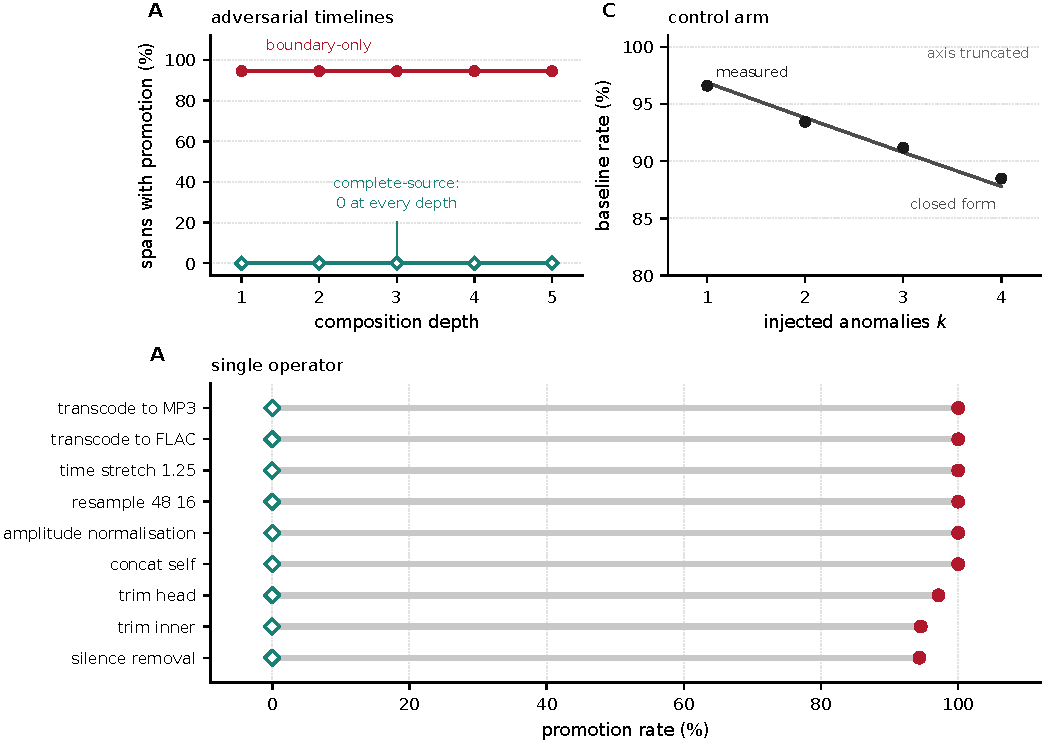
\includegraphics[width=0.88\linewidth]{fig3_promotion.pdf}
\caption{Boundary-only versus complete-source inheritance on \Btimelines{}
deterministic timelines. (A) Promotion does not grow with composition depth,
because the loss is established at the first derivation and no downstream
operator can recover evidence already discarded. (B) Each operator applied
alone, as a pair of marks per row: filled circles are boundary-only, open
diamonds are complete-source. Complete-source is zero for every operator and is
drawn as a mark rather than as a bar of no extent, so that a zero reads as the
result it is and not as missing data. (C) Control arm with anomaly positions
uniform over all positions, measured against the closed form
$\binom{n-2}{k}/\binom{n}{k}$. Its vertical axis is truncated to 80--100\%,
marked on the panel, so that any divergence between measurement and prediction
is visible rather than compressed; the truncation exposes prediction error and
is not a prevalence estimate. Percentages throughout quantify mechanism stress
on a frozen fixture family and are not real-world prevalence.}
\label{fig:promotion}
\end{figure}

\subsection{Which shortcut matters: a policy ablation}
\label{sec:res-ablation}

The baseline combines two shortcuts, and removing them one at a time over
\ABcases{} timelines per arm gives an unambiguous answer
(Table~\ref{tab:ablation}). In the \emph{interior} arm the anomaly lies inside
the nominal represented range, so only the inheritance axis can see it: both
boundary-only policies promoted on every timeline (\BZeroInterior{} and
\BOneInterior{}) and both complete-source policies on none. In the
\emph{footprint} arm the anomaly lies just outside the nominal range but inside
the declared kernel footprint: both footprint-blind policies promoted on every
timeline (\BZeroFootprint{} and \BTwoFootprint{}) and both footprint-aware
policies on none. Neither axis is redundant and neither is sufficient, which
is the argument for specifying them together.

\begin{table}[t]
\centering
\caption{Policy ablation over \ABcases{} timelines per arm. The interior arm
places the anomaly inside the nominal represented range; the footprint arm places
it outside that range but inside the declared kernel footprint. Each shortcut
fails exactly one arm, and only the full contract clears both.}
\label{tab:ablation}
\small
\begin{tabular}{llccc}
\toprule
Policy & Inheritance & Kernel footprint & Interior anomaly & Footprint anomaly \\
\midrule
B0 & boundary-only & no & 10\,000 (100\%) & 10\,000 (100\%) \\
B1 & boundary-only & yes & 10\,000 (100\%) & 0 (0\%) \\
B2 & complete-source & no & 0 (0\%) & 10\,000 (100\%) \\
B3 & complete-source & yes & 0 (0\%) & 0 (0\%) \\
\bottomrule
\end{tabular}

\end{table}

\subsection{Mixed-origin audio through stock FFmpeg}
\label{sec:res-corpus}

On \Cclips{} clips, complete-source propagation recovered the evidence
interval structure exactly, every boundary at sample resolution, for \Cexact{}
clips, and identified the generated interval with its exact bounds for \Cgen{},
with no detector, no training and no acoustic feature. The ground truth is
constructed rather than discovered: the question is
whether evidence originating at the capture and generation steps
\emph{survives} a chain of representation-only transformations, not whether it
could be inferred from the signal, and nothing here supports a claim that
generated audio can be identified without evidence. The robustness arm behaves
identically: \CtwoNeuralExact{} of \CtwoNeuralN{} neural-TTS clips and
\CtwoNoiseExact{} of \CtwoNoiseN{} noise-buried clips recovered their full
interval structure, with \CtwoNeuralEm{} and \CtwoNoiseEm{} promotions; under
the noise overlay the captured segments correctly become \textsc{mixed} while
the generated segment stays \textsc{generated}, since union adds no atom.
Boundary-only inheritance promoted the whole-asset claim to captured-only on
\Cbase{} clips and omitted required lineage on \CbaseLineage{}; the
complete-source policy produced \Cem{} promotions and \CemLineage{} omissions.

Across \Dtransforms{} transformations and \Druns{} runs
(Figure~\ref{fig:corpus}; Table~\ref{tab:main}), boundary-only inheritance
promoted on \Dbase{} runs and complete-source propagation on \Dem{}, with
\DemLineage{} lineage omissions. Two transformations produced \emph{no}
baseline promotion, and we report that as readily as the rest: overlay declares
the generated source as a separate top-level ingredient, so a boundary-only
reading still sees both, and silence removal happened to retain runs whose
boundaries fell inside the generated region.

The interval model was validated against FFmpeg's actual output on every PCM
run and on a \DdetermN{}-clip subset for the coded containers. The largest
deviation between predicted and actual output sample count was \DsilenceDev{}
samples for silence removal, \DstretchDev{} for time stretching,
\DmpThreeDev{} for MP3 and \DresampleDev{} for resampling; for \DguardOK{}
transformations the declared mapping margin covered it. That measurement
validates the \emph{mapping and alignment} of the interval model and not the
\emph{support containment} Proposition~\ref{prop:footprint} requires, because
an operator can emit exactly the predicted number of samples while depending
on sources outside the declared footprint; containment is tested directly in
Section~\ref{sec:res-containment}. Re-running each transformation and comparing
decoded essence gave \Ddeterm{} mismatches, so the processing path is
deterministic on this machine. The zero promotion count follows from Proposition~\ref{prop:union} once the
required source set is correct, and on overlay, during development, it did not;
the falsifiable measurements are the mapping deviation and margin coverage
here, and support containment in Section~\ref{sec:res-containment}.

\begin{figure}[tbp]
\centering
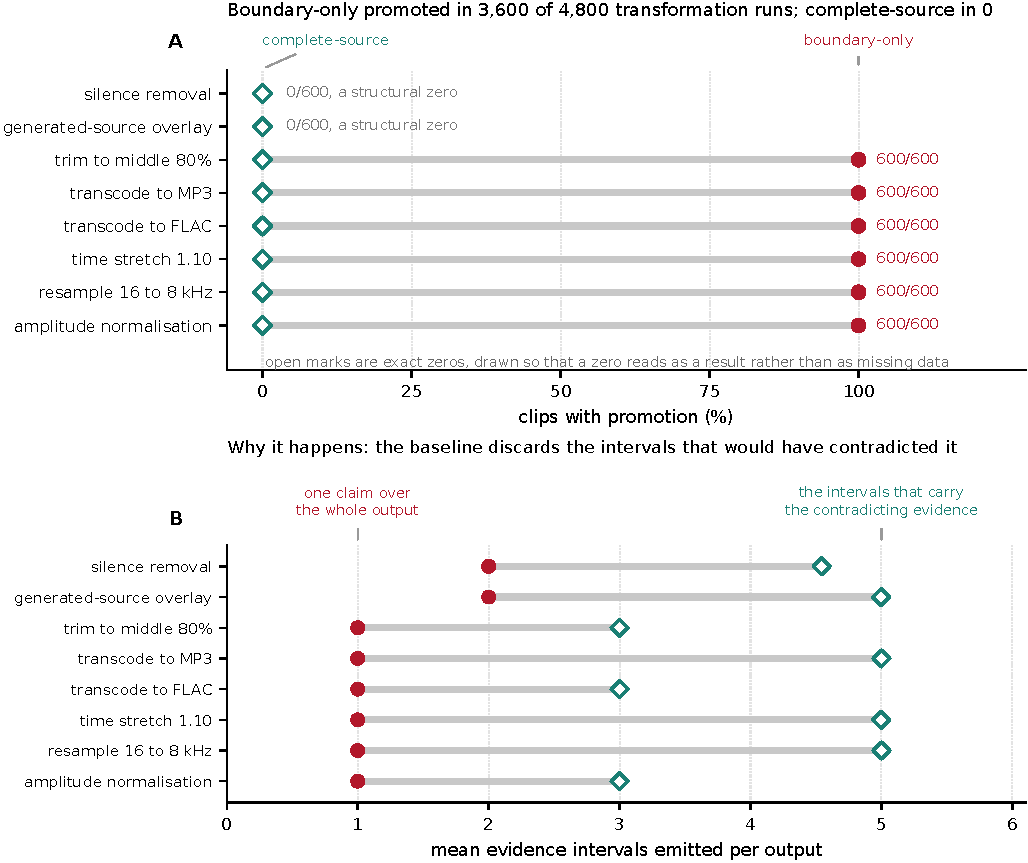
\includegraphics[width=0.82\linewidth]{fig4_corpus.pdf}
\caption{Promotion by transformation over \Cclips{} mixed-origin clips
processed entirely by stock FFmpeg, \DtotalRuns{} transformation runs in all.
Each row is a pair of marks: a filled circle for the boundary-only reference
policy and an open diamond for complete-source propagation, with counts written
directly rather than read off the axis. Boundary-only promoted in
\DbasePromo{} of \DtotalRuns{} runs and complete-source in \DemPromo{}.
Generated-source overlay and silence removal produce no baseline promotion
either, for the structural reasons given in Section~\ref{sec:res-corpus}, and
are marked as such rather than left to look like missing rows. (B) The mechanism
behind panel A, measured in the same runs: the mean number of evidence intervals
each policy emits per output. Boundary-only inheritance emits one interval for
most transformations, a single claim spanning the whole output, while
complete-source propagation emits three to five. The promotion in panel A is a
consequence of that collapse, since an interval that no longer exists cannot
carry the evidence that would have contradicted the endpoints. The baseline is a
constructed reference policy, not the behaviour of any named deployed product,
and these are counts over a frozen corpus rather than a prevalence estimate.}
\label{fig:corpus}
\end{figure}

\subsection{Signed transport, derivation and provenance loss}
\label{sec:res-transport}

Across \Ftotal{} signed round-trips over \Fcontainerlist{}, \Fclips{} clips
per container, signing succeeded and validation reported the
trusted state under the declared local anchor for \Ftrusted{} assets, with
\Fvalfail{} validation failures. The EM assertion returned byte-equivalent from
the validator for \Fassertion{} assets. After derivation with stock FFmpeg,
re-signing with the parent as an ingredient, and re-validation, \Fderived{}
derived assets validated and \Fparent{} recorded the \texttt{parentOf}
relationship.

Signal transparency holds exactly. Decoded essence was identical before
signing, after signing with the complete-source assertion and after signing
with the baseline assertion, with \Fmismatch{} mismatches against the
pre-signing essence and \FmismatchPolicy{} between policies. The whole-file hash changed in \Ffilechanged{} of \Ftotal{} cases, which is
why the comparison is defined on decoded PCM; a clean-clone rerun makes the
same point, every essence hash agreeing and no signed-file hash, each
signature carrying its own timestamp.

Under the five provenance-loss conditions over \Eclips{} clips, a valid
manifest yielded \textsc{mixed} in \Evalid{} cases, a removed manifest yielded \textsc{unverified} in
\Estripped{} cases, an asset modified after signing yielded \textsc{invalid} in
\Etampered{}, and re-encoding without manifest preservation yielded
\textsc{unverified} in \Ereenc{}. No condition other than a valid manifest ever
yielded \textsc{captured}, and there were \Eviol{} violations of the
classification requirement. We do not claim that stripping is detected as
malicious intent; the result is that the classification degrades in the
conservative direction.

\subsection{Kernel-support containment}
\label{sec:res-containment}

\begin{figure}[tbp]
\centering
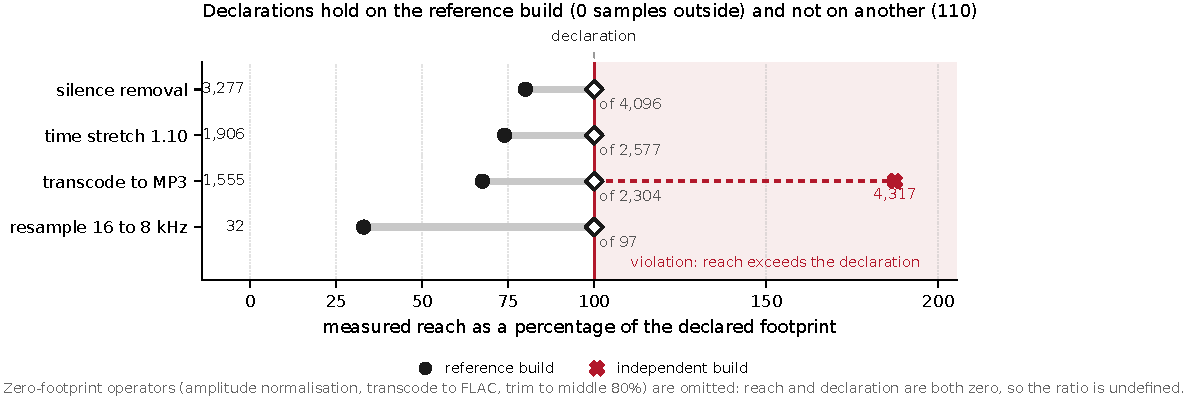
\includegraphics[width=0.88\linewidth]{fig5_containment.pdf}
\caption{Kernel-support containment. Each operator configuration was probed
with a proportionate single-sample impulse at ten prespecified positions in each
of \Kcontexts{} deterministic signal contexts, \Kprobes{} probes in total.
Filled circles are the furthest any one source sample was measured to influence
the output beyond the nominal source range on the reference build; open diamonds
are the declared footprint; crosses are the same measurement on the independent
reproduction's FFmpeg (Section~\ref{sec:res-independent}), shown wherever the
two builds disagree. The axis is the measurement as a percentage of its own declaration,
because the operators span two orders of magnitude in samples and a shared
linear axis would hide the tightest row; absolute counts are given as direct
labels. Containment requires the measurement to fall at or left of its
declaration. On the reference build \KoutsideTotal{} influenced samples fell
outside. On the independent build the MP3 declaration does not contain its own
measurement: the reach is \IRmpReach{} source samples against \IRmpDeclared{}
declared, which is the mark in the shaded band, and \IRmpOutside{} output
samples fall outside the declared support. That row is the paper's own
counterexample to treating these numbers as portable. Silence
removal is the reason this experiment exists: an earlier declaration was
exceeded, the probe detected it, and the band was raised to \KsilenceFp{}
samples. These are measurements of the frozen configurations tested, not
universal codec constants.}
\label{fig:containment}
\end{figure}

Proposition~\ref{prop:footprint} needs the declared required-source set to
contain the actual dependency set, a statement about which source samples
influence which output samples, not about how many output samples there are.
We test it directly on the \Kops{} single-source
configurations; concatenation and overlay take several sources and have no
temporal kernel to under-declare. For
each configuration, each of \Kcontexts{} signal contexts and each of ten probe
positions, two \KimpulseN{}-sample sources are built that are identical except
at one sample, where one carries an added impulse; both go through the same
stock FFmpeg command and both outputs are decoded, so the entire difference
between the paired outputs is attributable to that one sample. Containment
holds when the probe position lies inside the declared required-source range of
every output sample whose value it changed, on 16-bit PCM at a threshold of one
least significant bit.

Two properties of the probe had to be got right, and getting them wrong first
showed why: against silence every operator appears to map one sample to one
sample, and an earlier fixed-amplitude impulse, roughly two hundred times the
carrier in the low-level context, replaced an adaptive operator's input rather
than perturbing it, so both the lossy encoder and the stretcher re-decided
globally. The impulse is now a fixed multiple of each context's peak. The
\Kcontexts{} contexts, all generated arithmetically
(\texttt{experiments/support\_containment.py}), are a steady low-frequency
tone; the same tone at one part in a hundred, where a lossy encoder allocates
fewest bits; sharp onsets with exponential decay, which drive an overlap-add
stretcher hardest; and six inharmonic partials, where masking is most active. Lossy
transcoding spreads a single source sample across up to \KmpThreeSpread{}
output samples at every position, resampling across up to \KresampleSpread{},
and overlap-add stretching is strongly position-dependent, reaching up
to \KstretchSpread{} at the \KstretchAboveOne{} probes inside an overlap
region and one sample elsewhere, which is why the test is run against the
worst case rather than the median.

Across \Kprobes{} probes, \Kaffected{} output samples were influenced and
\Koutside{} fell outside the declared support (Table~\ref{tab:containment};
Figure~\ref{fig:containment});
every context produced influence for every operator, so no row passes
vacuously. That zero was not free. A shorter probe passes trivially for the
large-footprint operators because a declared footprint of \KstretchFp{} samples
spans a whole short source; lengthening it made the test able to fail, and it
did. Silence removal failed: a frame-granular selector emitted a frame
beginning \KsilenceReach{} source samples before a retained run's start, well
beyond the margin declared at the time. That is an under-declaration, the one
direction Proposition~\ref{prop:footprint} does not forgive; the band was
raised to \KsilenceFp{}, above the measured reach, and the operator now
contains with a margin of \KsilenceMargin{}. We report this rather than
quietly shipping the corrected number because it is the clearest evidence that
the bounds are measured rather than asserted. The bands are also reasonably
tight, which matters because a larger one would be equally safe and more
dilutive: resampling reached \KresampleReach{} against \KresampleFp{}, MP3
\KmpThreeReach{} against \KmpThreeFp{}, and time stretching \KstretchReach{}
against \KstretchFp{}.

\begin{table}[t]
\centering
\caption{Kernel-support containment. Probed as Figure~\ref{fig:containment}
describes. The measured reach is the furthest any influence extended
beyond the nominal, footprint-free source range, so containment compares two
concrete quantities rather than resting on an assertion: it holds exactly when
the reach does not exceed the declaration. Headroom is the difference, so a
small headroom means a tight declaration and a large one a conservative one.
$^{\dagger}$~Amplitude normalisation's declared footprint is
\emph{representational}: an output sample represents one source sample, while
the scalar gain depends computationally on the whole signal. The probe therefore
confirms the representational reading and does not show that the computational
dependency is zero, which it is not.}
\label{tab:containment}
\small
\begin{tabular}{lrrrrr}
\toprule
Operator & Declared & Measured reach & Influenced samples & Headroom & Outside \\
\midrule
amplitude normalisation$^{\dagger}$ & 0 & 0 & 40 & 0 & 0 \\
resample 16 to 8 kHz & 97 & 32 & 1\,131 & 65 & 0 \\
silence removal & 4\,096 & 3\,277 & 28 & 819 & 0 \\
time stretch 1.10 & 2\,577 & 1\,906 & 10\,971 & 671 & 0 \\
transcode to FLAC & 0 & 0 & 40 & 0 & 0 \\
transcode to MP3 & 2\,304 & 1\,555 & 39\,763 & 749 & 0 \\
trim to the middle 80\% & 0 & 0 & 32 & 0 & 0 \\
\bottomrule
\end{tabular}

\end{table}

\subsection{C2PA-native heterogeneous composition}
\label{sec:res-composition}

The strongest form of the standards argument is executable. For \Jfixtures{}
fixtures, a captured source and a generated source are each signed with their
own \texttt{digitalSourceType}; stock FFmpeg concatenates them; the
composition is signed with both sources as \texttt{componentOf} ingredients
carrying their full manifests, a \texttt{c2pa.placed} action referencing each,
and the EM assertion computed over the two component timelines; it is then
derived across the ancestry boundary and re-signed with \texttt{parentOf}.

\texttt{c2pa.mixed} is defined for
``multiple, previously placed (via \texttt{c2pa.placed} actions) audio
ingredients (e.g., stems, vocals, drums, bass, etc) [that] are combined and
optionally transformed'' \citep[Table~8]{c2pa24}. Our fixture concatenates in sequence rather than summing, and we read that as
placement rather than mixing, a \emph{documented profile decision} rather than
a normative one, since the specification settles neither that nor
\texttt{c2pa.remixed} \citep[Table~8]{c2pa24}. \texttt{c2pa.mixed}
presupposes \texttt{c2pa.placed}, so the placed actions are required under any
reading, and the choice does not affect the contract, which reads the
ingredient graph and the interval map, not the action label.

All \Jfixtures{} compositions validated as trusted under the declared anchor,
with both \texttt{componentOf} ingredients recorded in \Jcomponents{} cases and
both \texttt{c2pa.placed} references resolved in \Jplaced{}; the EM assertion
returned byte-equivalent in \Jroundtrip{}; the whole-asset aggregate was
\textsc{mixed} with both intervals individually recoverable in \Jmixed{}; and
the derived asset stayed \textsc{mixed} and trusted in \JderivedMixed{} of
\JderivedTrusted{} derivations, with \Jessence{} essence mismatches. This is
the object the vocabulary-versus-reduction distinction describes: the component
histories are all present in the signed graph, and the aggregate interval claim
exists only because the EM assertion computes it. Nothing in the validation
pipeline required it to be conservative. A representative manifest is frozen
as a fixture in the repository.

\subsection{The cost of conservatism: claim dilution}
\label{sec:res-dilution}

\begin{figure}[tbp]
\centering
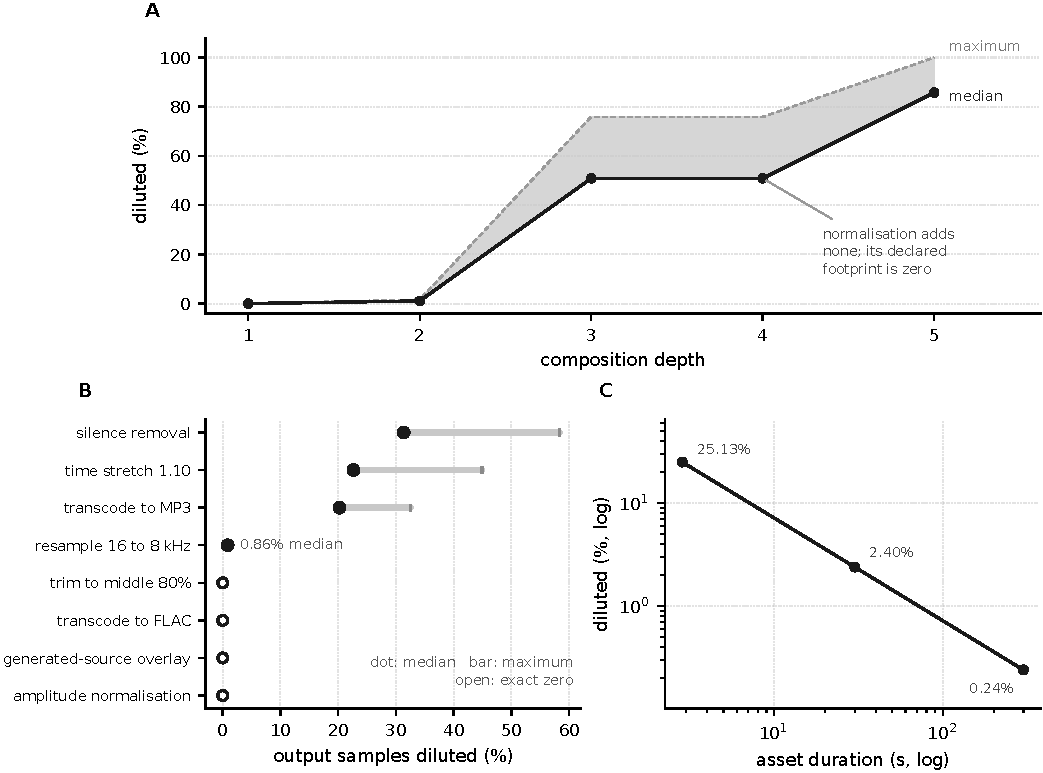
\includegraphics[width=0.84\linewidth]{fig6_dilution.pdf}
\caption{What the declared footprints cost. (A) Dilution through a composition
chain, median with the maximum envelope. The cost compounds with depth and is
the headline of this figure, which is why it takes the full width. The plateau
at depth four is amplitude normalisation, whose declared representational
footprint is zero and which therefore adds none. (B) Dilution for a single
transformation over \IclipsPerTf{} clips: filled circles are medians, bars
reach the maximum, and open circles are exact zeros drawn as marks so that a
zero is legible as a result rather than as missing data. (C) The same
depth-three chain over three asset durations on logarithmic axes, showing that
fixed-width bands occupy a smaller fraction of a longer asset. Panel C holds the
chain and the boundary count fixed and is not a claim about arbitrary chains:
more ancestry boundaries would place more bands. Dilution is a weaker claim over
part of an asset, never a stronger one, so this is the price of conservatism and
not a failure mode.}
\label{fig:dilution}
\end{figure}

Zero promotion is only half of a useful result, because safety alone is cheap:
declaring the whole asset as every sample's dependency is perfectly safe under
Proposition~\ref{prop:footprint} and perfectly useless. We therefore measure
what the declared footprints cost. The \emph{dilution fraction} of a derived
output is the fraction of its samples whose footprint-aware evidence record is
strictly weaker, in claim, channel or support value, than the record computed
over the nominal represented content, which on this corpus is exact by
construction.

Measuring this caught a second defect in our own implementation, reported for
the same reason as the first. Footprint widening was originally applied at the
granularity of the emitted interval partition, so an interval whose widened
range touched a neighbouring ancestry took the weakened claim over its
\emph{entire} extent, and a single resampling reported a dilution fraction of
one: safe, and uselessly conservative. The fix refines the output partition at
the pull-backs of each source boundary shifted by $\pm$ the footprint, confining
dilution to footprint-wide bands at ancestry boundaries. The two-language
differential had not caught this because its fixtures used source intervals
narrower than every footprint, a geometry in which the coarse and exact
treatments coincide; the oracle corpus now includes a wide-interval battery,
and the fixed implementation agrees with the per-sample oracle on all
\Hcases{} cases.

After the fix (Table~\ref{tab:dilution}; Figure~\ref{fig:dilution}), \IzeroTf{} of \ItfCount{}
transformations dilute nothing, lossless transcoding among them, and overlay
because its nominal required-source set already contains every covering
source. The remainder
dilute the footprint-wide neighbourhood of each ancestry boundary: median
dilution is \IresampleMedianPct{}\% for resampling, \ImpThreeMedianPct{}\% for
MP3, \IsilenceMedianPct{}\% for silence removal and \IstretchMedianPct{}\% for
time stretching, with a single-transformation worst case of \ImaxAnyPct{}\%.
Each band has a \emph{fixed radius in samples} and the clips average
\CmeanDurS{}~s, so the same bands on a one-hour asset would occupy a fraction
three orders of magnitude smaller: the fraction shrinks with duration, the
absolute band does not.

Composition is where conservatism bites. Along the chain trim, resample 16 to
8~kHz, transcode to MP3, normalise, time stretch by 1.10, deliberately
front-loading a rate change so that the large bands are scaled by it, median
dilution reaches \IchainDeep{}\% by depth~\IchainDepth{} with a worst case of
\IchainDeepMax{}\%; depth~4 equals depth~3 to the last digit because the
operator added there, normalisation, has a zero footprint. Whether a rate change rescales upstream bands is not isolated by this design,
whose only rate change occurs before any upstream band exists. Holding a routine three-operator chain fixed (trim,
normalise, MP3) and varying only duration, dilution is \IlongShortPct{}\% at
the corpus median length, \IlongThirtyPct{}\% at 30~s and
\IlongThreeHundredPct{}\% at five minutes: each tenfold increase in duration
divides the fraction by ten, as fixed-width bands predict when the number of
boundaries is held fixed, which it is here and would not be for an arbitrary
chain. Dilution therefore dominates only where a deep chain of large-footprint
operators meets a short asset with many ancestry boundaries, which is what this
measurement deliberately constructs; the quantity a deployment should carry is
the band radius of Table~\ref{tab:operators}, not a percentage measured on
\CmeanDurS{}-second clips. This is the price of declaring conservative bounds
instead of knowing exact codec dependencies, and it can be bought back without
losing safety: any tighter map that remains an over-approximation reduces
dilution and, by Proposition~\ref{prop:footprint}, cannot introduce
promotion.

\begin{table}[t]
\centering
\caption{Claim dilution: the fraction of output samples whose footprint-aware
evidence is strictly weaker than the evidence over the nominal represented
content, per transformation over \IclipsPerTf{} clips and along a composition
chain over \IchainClips{} clips. This is the price of the declared footprints,
which combine analytical support with implementation margin, when the nominal map
is exact.}
\label{tab:dilution}
\small
\begin{tabular}{lrrrr}
\toprule
Transformation & Clips & Median dilution & Max dilution & Clips affected \\
\midrule
amplitude normalisation & 600 & 0.00\% & 0.00\% & 0 \\
overlay a generated source & 600 & 0.00\% & 0.00\% & 0 \\
resample 16 to 8 kHz & 600 & 0.86\% & 1.39\% & 600 \\
silence removal & 600 & 16.48\% & 32.80\% & 600 \\
time stretch 1.10 & 600 & 22.64\% & 44.92\% & 600 \\
transcode to FLAC & 600 & 0.00\% & 0.00\% & 0 \\
transcode to MP3 & 600 & 20.24\% & 32.56\% & 600 \\
trim to the middle 80\% & 600 & 0.00\% & 0.00\% & 0 \\
composition depth 1 & 200 & 0.00\% & 0.00\% & --- \\
composition depth 2 & 200 & 1.06\% & 1.59\% & --- \\
composition depth 3 & 200 & 50.87\% & 75.84\% & --- \\
composition depth 4 & 200 & 50.87\% & 75.84\% & --- \\
composition depth 5 & 200 & 85.74\% & 99.99\% & --- \\
30\,s asset, depth-3 chain & 1 & 2.40\% & --- & --- \\
300\,s asset, depth-3 chain & 1 & 0.24\% & --- & --- \\
\bottomrule
\end{tabular}

\end{table}

\subsection{Two-language differential}
\label{sec:res-oracle}

The Python reference implementation works with interval algebra over pulled-back
source boundaries; the Node.js oracle evaluates evidence per output sample by
brute force and run-length-encodes the result, with no interval algebra at all.
The frozen corpus spans footprints wider than every source interval and
footprints far narrower, the regime added after the dilution experiment
(Section~\ref{sec:res-dilution}). It is stored as
\path{fixtures/oracle_cases.jsonl}, one case per line carrying the interval
model and the source evidence in a form that names neither implementation,
and the oracle reads it as a separate process. On \Hcases{} cases the two agreed
on interval structure, provenance state, lineage set and channel availability
with \Hdis{} disagreements, and the maximum absolute difference in any support
value was \Hdelta{}. Both implementations are author-written, so this is a
differential test against transcription and interval-arithmetic error, not
evidence of independence from the author (Section~\ref{sec:limits}).

\subsection{Cost}
\label{sec:res-overhead}

Complete-source bookkeeping cost a median \Gem{}~ms per audio-minute against
\Gbase{}~ms for boundary-only, a ratio of \Gratio{}$\times$ computed from the
unrounded medians, and \GffmpegPct{}\% of the FFmpeg time it accompanies
(Table~\ref{tab:overhead}). Signing took a median
\Gsign{}~ms per asset (IQR \GsignQa{}--\GsignQb{}) and validation \Gval{}~ms
(IQR \GvalQa{}--\GvalQb{}). Manifest overhead was \Gmanifest{}~B per asset, of
which the EM assertion was \Gassertion{}~B; the fixed per-asset component
(certificate chain, COSE structure, hard binding) dominates, and the variable
part grows linearly in emitted evidence intervals at \GperInterval{}~B and
\GperIntervalUs{}~$\mu$s per interval, measured up to \GmaxIntervals{} with no departure from linearity. Cost
therefore scales with how often ancestry changes along the timeline, not with
duration. It also scales with how far the codec smears that ancestry: the
assertion is \FassertionWav{}~B in \texttt{wav} and \FassertionFlac{} in
\texttt{flac} against \FassertionMpThree{} in \texttt{mp3}, whose footprint
splits it into more intervals. An implementation that wants a ceiling on the count may coarsen the
partition, merging adjacent intervals and emitting the meet over the merged
range: each sample then carries the union of the merged required source sets,
which by Proposition~\ref{prop:footprint} can only weaken its claim, at the
dilution cost of Section~\ref{sec:res-dilution}. The byte figure is deterministic and reproduces exactly; the
microsecond figure is wall clock on one interpreter and one machine.

Of these figures the ratio travels and the milliseconds do not, and the
mechanism is structural: both arms are timed in the same process on the same
machine, so thermal state, clock frequency or competing load moves them
together and cancels in the quotient. Re-running the benchmark as
\MstabRepeats{} independent processes gives the absolute cost a coefficient of
variation of \MstabAbsPct{}\% against \MstabRatioPct{}\% for the ratio, with
the per-process rows and their load averages in Supplementary
Note~\NoteRawRows{}; across sittings on this machine the absolute figure has
moved by about a third while the ratio stayed inside its band. On a quiet machine with little common mode to cancel the quotient can carry
slightly more scatter than either arm, and we have observed both cases.
Cancelling variation within a machine is not cancelling the difference between
two, so the cross-machine question is settled by measurement in
Section~\ref{sec:res-independent}: the absolute figure differs by
\IRabsGap{}\% and the ratio by \IRratioGap{}\%. The milliseconds are
order-of-magnitude evidence that the bookkeeping is cheap, not reproducible
constants.

\begin{table}[t]
\centering
\caption{Main results. Deterministic fixture rates characterise the frozen
fixture family and are a mechanism stress rate, not a population prevalence
estimate.}
\label{tab:main}
\small
\begin{tabular}{lrrr}
\toprule
Check & Cases & Boundary-only & Complete-source \\
\midrule
\multicolumn{4}{l}{\textit{A\quad Exhaustive finite-state conformance}} \\
Source words over $\{C,G,\bot\}$, length $\le 8$ & 9,840 & --- & --- \\
Operator cases & 98,385 & --- & --- \\
Contract checks & \multicolumn{3}{l}{885,828 checks, 0 failed} \\
Named regression tests & \multicolumn{3}{l}{30 tests, 30 passed, 0 failed} \\
\addlinespace
\multicolumn{4}{l}{\textit{B\quad Deterministic adversarial timelines (10\,000 frozen fixtures, 64 intervals)}} \\
Chain depth 1 & 10,000 & 9,455 (94.5\%) & 0 \\
Chain depth 3 & 10,000 & 9,455 (94.5\%) & 0 \\
Chain depth 5 & 10,000 & 9,455 (94.5\%) & 0 \\
Lineage omissions (depth 1) & 10,000 & 10,000 & 0 \\
Unverified $\to$ verified (depth 1) & --- & 7,222 & 0 \\
\addlinespace
\multicolumn{4}{l}{\textit{C--D\quad Mixed-origin audio corpus, stock-FFmpeg processing}} \\
Exact propagation of constructed interval evidence & 600 & --- & 600 \\
amplitude normalisation & 600 & 600 (100.0\%) & 0 \\
overlay a generated source & 600 & 0 (0.0\%) & 0 \\
resample 16 to 8 kHz & 600 & 600 (100.0\%) & 0 \\
silence removal & 600 & 0 (0.0\%) & 0 \\
time stretch 1.10 & 600 & 600 (100.0\%) & 0 \\
transcode to FLAC & 600 & 600 (100.0\%) & 0 \\
transcode to MP3 & 600 & 600 (100.0\%) & 0 \\
trim to the middle 80\% & 600 & 600 (100.0\%) & 0 \\
\addlinespace
\multicolumn{4}{l}{\textit{H\quad Two-language differential oracle}} \\
Frozen cases & 10,860 & --- & 0 disagreements \\
\bottomrule
\end{tabular}

\end{table}

\begin{table}[t]
\centering
\caption{Cost, as medians over \Greps{} repetitions on one machine. These are
measurements of a Python reference implementation, not language-independent
constants.}
\label{tab:overhead}
\small
\begin{tabular}{lll}
\toprule
Quantity & Median & IQR \\
\midrule
EM bookkeeping & 1.345 ms / audio-minute & 1.336--1.390 ms / audio-minute \\
Boundary-only bookkeeping & 0.406 ms / audio-minute & 0.403--0.412 ms / audio-minute \\
EM $/$ boundary-only ratio & 3.31$\times$ & --- \\
EM as a fraction of FFmpeg time & 0.148\% & --- \\
C2PA signing & 17.2 ms / asset & 16.8--17.9 \\
C2PA validation & 14.1 ms / asset & 14.0--14.6 \\
Manifest size overhead & 14,932 B / asset & 14,932--14,933 \\
EM assertion & 1,333 B / asset & 1,333--1,334 \\
EM assertion marginal cost & 333 B / evidence interval & --- \\
\bottomrule
\end{tabular}

\end{table}

\begin{table}[tbp]
\centering
\caption{Claim--evidence boundary and what transfers. Each row names a class of
claim, the evidence used for it, what that evidence does not establish, and whether
the independent reproduction of Section~\ref{sec:res-independent} reproduced
it. Evidence from one row is
never used to authorise a claim in another.}
\label{tab:boundary}
\footnotesize
\begin{tabular}{p{0.14\linewidth}p{0.26\linewidth}p{0.24\linewidth}p{0.23\linewidth}}
\toprule
Claim class & Evidence used here & Not established by it & Transfers? \\
\midrule
Operator conformance &
Propositions~\ref{prop:union} and~\ref{prop:footprint} and
Theorem~\ref{thm:composition}; exhaustive enumeration; \LscopeCases{}-case
scope battery; \Hcases{}-case two-language differential &
That any deployed system conforms; the prevalence of non-conformance &
Yes: proved from the requirements; \IRachecks{} checks of the suite he was
given, \IRafailed{} failures; the current \Achecks{} reproduced exactly by the
Windows run of tag~\XBWinTag{}; scope and oracle cases reproduced exactly \\
\addlinespace
Mechanism on constructed fixtures &
\Btimelines{} frozen adversarial timelines with a closed-form control arm &
Any population rate; the behaviour of any named product &
Yes: \BbaseOne{} baseline promotions against \BemAll{}, reproduced exactly \\
\addlinespace
Mechanism on realistic audio &
\Cclips{} labelled mixed-origin clips processed by stock FFmpeg &
Balanced coverage of speakers, languages, codecs or editing styles &
Yes: \DemPromo{} promotions against \DbasePromo{}, reproduced exactly \\
\addlinespace
Interval-model fidelity &
Predicted versus actual output sample counts on every PCM run and a
\DdetermN{}-clip coded subset, against declared margins &
Kernel-support containment, a different property; the margins on other
codecs, builds or configurations &
\textbf{No}: silence-removal deviation rises from \IRsilDevRef{} to
\IRsilDev{} samples against a \IRsilGuard{}-sample margin \\
\addlinespace
Kernel-support containment &
\Kprobes{} probes: ten positions in each of \Kcontexts{} contexts across
\Kops{} operator configurations, on decoded PCM at one least significant bit &
Containment at untested positions, signals, codecs or configurations; the
operators as configured here, not the operator class; which configuration
produced a given asset, which the assertion does not record &
\textbf{No}: the MP3 declaration is under-sized on the other build, reach
\IRmpReach{} against \IRmpDeclared{} \\
\addlinespace
Signed transport and signal transparency &
\Ftotal{} round-trips through the official tool over
\Fcontainerlist{}; decoded-PCM SHA-256 identity under both policies &
Conformance-program trust; security of the C2PA cryptographic layer;
perceptual equivalence; bit-exactness across decoders; any container the
signing tool accepts but this experiment did not carry &
Yes: identical before and after signing on both machines \\
\addlinespace
Consumer-side verification &
Per-interval lineage and the ingredient graph, both returning
byte-equivalent through the official tool
(Sections~\ref{sec:res-transport}, \ref{sec:res-composition}) &
Detection of promotion: the assertion records an operator, not the chain,
so a consumer cannot recover the required source set &
\textbf{No} for detection; the schema omits it, not the build \\
\addlinespace
Runtime cost &
\Greps{} timed repetitions on one declared machine &
Cost in a compiled implementation or at broadcast scale &
\textbf{No} for milliseconds, \IRabsGap{}\% apart and \IRabsCv{}\% dispersed
within one sitting; approximately for the ratio, \IRratioGap{}\% apart on one
pair of machines \\
\addlinespace
Conservatism cost &
Per-sample dilution against constructed exact ground truth &
Dilution against the true, unknowable dependencies of a third-party codec &
Yes: reproduced exactly \\
\bottomrule
\end{tabular}
\end{table}

\subsection{Independent reproduction}
\label{sec:res-independent}

The classification of outputs was fixed in code and shipped before any third
party ran it (Section~\ref{sec:limits}), so what follows is a protocol
executed rather than a comparison arranged after the fact.

D.~A.~Balderrama-Alvarez (Universidad de Sonora) ran the package for release
tag~\IRtag{} twice on his own machine (Table~\ref{tab:runs}). He is not an author, took no part in designing the contract
or the experiments, and received the package without any result files: this is
independence of execution, not of implementation (Section~\ref{sec:limits}).
The first run was incomplete because two dependencies were absent from the
package's instructions, since fixed; the second, reported here, produced the
same values for the two findings below, which rules out run-to-run variation
on his hardware. The package he was
given, tag~\IRtag{}, is earlier than the released \Rtag{}; neither finding's
value changed between the two, which we checked rather than assumed, and what
did change is the size of the conformance suite, as recorded below. His raw
outputs are released unmodified in \texttt{results/independent/}.

\path{tools/verify_reproduction.py} returned \texttt{REPRODUCTION
INCOMPLETE} with the \IRdet{} differences reported below, and
\texttt{run\_all.sh} ended in \texttt{RUN FAILED} for two packaging defects
that touch no reported number (Supplementary Note~\NoteRepro{}). Both are printed because Section~\ref{sec:limits} makes that tool the arbiter
precisely so its verdict cannot be adjusted after the fact.


\begin{table}[tbp]
\centering
\caption{The reference machine and the three third-party runs. \emph{MP3
reach} is the measured kernel reach in source samples against a declared
footprint of \IRmpDeclared{}. The reference and two of the runs use
FFmpeg~\Vffmpeg{}; those two are different builds of that one version and do
not agree, which is why the declaration is stated per build. Full
environments and per-operator detail are Supplementary
Note~\NoteIndependent{}.}
\label{tab:runs}
\footnotesize
\begin{tabular}{p{0.19\linewidth}p{0.13\linewidth}p{0.17\linewidth}p{0.27\linewidth}p{0.09\linewidth}}
\toprule
Run & Platform & FFmpeg & Verifier outcome & MP3 reach \\
\midrule
Reference (this paper) & \Vos{} & \Vffmpeg{} & --- & \XBRefReach{} \\
\addlinespace
D.~A.~Balderrama-Alvarez & \IRos{} & \IRffmpeg{} &
\texttt{REPRODUCTION INCOMPLETE}; \IRdet{} deterministic differences &
\IRmpReach{} \\
\addlinespace
B.~C.~Guerra Flores & \XBMacOs{} & \XBMacFfmpeg{} &
Exit zero; \XBMacEnvDiffs{} differences, all timings & \XBMacReach{} \\
\addlinespace
D.~A.~Balderrama-Alvarez & \XBWinOs{} & \XBWinFfmpeg{} &
\XBWinDetDiffs{} deterministic differences & \XBWinReach{} \\
\bottomrule
\end{tabular}
\end{table}

\paragraph{What reproduced} Of the \IRfiles{} result files carrying a
deterministic claim, \IRclean{} reproduced with no deterministic difference,
across an operating system, processor architecture, Python version and FFmpeg
major version that share nothing with the reference machine. Every headline
outcome is among them, including the \LscopeFailBad{} cases the superseded
rule failed, and Table~\ref{tab:boundary} reports them row by row.
Decoded-essence identity before and after signing held for all \Ftotal{}
round-trips; the digests differ between machines, as a different FFmpeg decodes
to different bytes, and the claim is identity within a machine.

\paragraph{What did not, and why it is a result} \IRdet{} deterministic
differences remain, in \IRdiffFiles{} files. \IRdetSuite{} of them are the size
fields of Experiment~A and are not a failing check: his package's suite had
\IRachecks{} checks and every one passed, and the released suite has
\Achecks{} because the structural checks were added after his run; the later
Windows run of tag~\XBWinTag{} reproduces the \XBWinChecks{} exactly, and every
deterministic output of that tag is identical to that of the evaluated release,
\Rtag{}. The
remaining \IRdetBuild{} fall in two files and trace to the same cause, the one
Section~\ref{sec:limits} names in advance: the kernel footprints of
Table~\ref{tab:operators} are declarations calibrated against one FFmpeg build,
and his is a different one.

\IRopsAgree{} of the \IRopsNonzero{} operators that declare a non-zero footprint
reproduced their measured reach exactly across the two builds; the remaining
\IRopsZero{} declare no footprint and measure no reach on either machine, so
their agreement carries no information. The supplement gives the per-operator
comparison in full.

For the MP3 encoder, the declared footprint of \IRmpDeclared{} source samples
was adequate on the reference build, where the measured reach was
\IRmpReachRef{}. On his build the reach is \IRmpReach{}, exceeding the
declaration by \IRmpExcess{}, and \IRmpOutside{} output samples fall outside
the declared support, all in the \IRmpContext{} probe context. This is a failure of one declared number, not of
Proposition~\ref{prop:footprint}, which covers enlargement and not
under-sizing, and its consequence is exactly the failure this paper is about: a
source's genuine influence reaches samples the assertion does not attribute to
it, which is promotion. An over-declared footprint costs dilution; an
under-declared one costs the guarantee, and a reader on an untested FFmpeg
build should assume the same until the calibration says otherwise.

For silence removal, the deviation between the modelled temporal mapping and
the one FFmpeg performs rises from \IRsilDevRef{} samples on the reference
build to \IRsilDev{} on his, against a declared margin of \IRsilGuard{}. The
median deviation is \IRsilMedian{}, a systematic offset rather than an outlier,
and \texttt{aselect} retains \IRsilLen{} samples on his build where the
reference retains \IRsilLenRef{}. His containment arm for this operator nonetheless
reported no sample outside the declared support: mapping and support are two
quantities validated by two experiments, and only the first failed.

\paragraph{Two builds, one version number} Two later runs on the released
package separate the version number from the environment around it
(Table~\ref{tab:runs}). The Guerra Flores run is the first by a third party to
reproduce every deterministic output of the package it ran; the Windows run's
\XBWinDetDiffs{} differences all lie in the MP3 kernel measurements and the
time-stretch model deviation, on which the two builds also disagree,
\XBRefStretchDev{} against \XBWinStretchDev{} samples, both inside the
\XBStretchGuard{}-sample margin.

What that supports is narrower than it may look. The version number is
\XBMacFfmpeg{} in three of the four rows and the reach takes two values, so
pinning a version is not a substitute for re-calibrating; machine and operator
do not move it, since the two runs that agree share neither. Operating system,
architecture and build differ together, so we claim only that the number is
not fixed by the version, and these runs were made to test the package rather
than as an experiment. The declaration of \IRmpDeclared{} samples contained
every measurement in this group, with \XBMacOutside{} and \XBWinOutside{}
probes outside.

We report the two findings on the Linux build as findings rather than as
reproduction failures, and we do not re-declare the numbers to make them pass:
widening them until his build conforms would produce a table adequate for two
builds and tested against neither. What the reproduction establishes is the
scope of Table~\ref{tab:operators}: a calibration for a stated configuration,
for which the re-calibration of Section~\ref{sec:limits} is a prerequisite and
the two-pass tool that performs it is the artefact that transfers.

That outcome is consistent with the broader forensic-tool literature without
validating anything here: \citet{nordvik2022exfat} showed that a shared
specification does not guarantee consistent interpretation across
implementations, while \citet{kuelper2026testdriven} showed that forensic
outputs can drift substantially across software versions. Our own runs add a
narrower observation: matching FFmpeg version strings do not guarantee
identical calibrated behaviour across builds. The contract is portable because
it is a proof; the calibrated constants are not, and are not assumed to be.

\paragraph{Cost, and which figure travels} His bookkeeping cost is \IRabs{}~ms
per audio minute against \IRabsRef{} on the reference machine, a difference of
\IRabsGap{}\%; the ratio to the baseline is \IRratio{} against \IRratioRef{}, a
difference of \IRratioGap{}\%. Within his sitting, across \MstabRepeats{} processes,
the absolute figure has a coefficient of variation of \IRabsCv{}\% against
\IRratioCv{}\% for the ratio, the shape Section~\ref{sec:res-overhead}
predicts: the quotient helps in proportion to the common-mode variation there
is to cancel. This is one pair of machines, so it shows the ratio surviving a
change of hardware once rather than bounding how far it can move.

\section{Discussion}
\label{sec:discussion}

\paragraph{What is established} That a complete-source rule is implementable
over media time against real processing software; that it eliminates promotion
on every fixture and corpus clip tested, where a minimal boundary-only policy
does not; that it can be carried in an existing signed standard without
altering the audio; and that its cost is a fraction of a percent of the
processing it accompanies. An independent run on unrelated hardware returned
the headline contract and corpus outcomes unchanged; of its \IRdet{}
deterministic differences, \IRdetSuite{} are the size of a suite that grew
after the run and \IRdetBuild{} trace to declarations his
FFmpeg build does not satisfy
(Section~\ref{sec:res-independent}). Independent execution shows those counts
are not artefacts of the reference machine; that they are properties of the contract follows from Propositions~\ref{prop:union}
and~\ref{prop:footprint} and Theorem~\ref{thm:composition}. Table~\ref{tab:boundary} states in one place what transfers:
everything derived from the requirements, and nothing derived from a
particular build, a boundary that runs through Table~\ref{tab:operators}.

\paragraph{What is not} No claim is made that any deployed system promotes
provenance; the baseline is a constructed reference policy and the fixture
rates are a mechanism stress rate. Nor is the algebra new: the non-amplification
property is a meet in a semilattice, familiar from provenance semirings
\citep{green2007provenance} and information-flow models
\citep{denning1976lattice,goguen1982noninterference}, and can equally be read as
a ``no write up'' discipline for evidential authority.

\paragraph{Relation to the standard and to adjacent work} The layer addressed
here is the reduction over a vocabulary that already preserves what the problem
needs, and it requires no specification change
(Section~\ref{sec:transport}). It has not been put to the C2PA working group
and no endorsement is claimed; standardisation of the reduction, rather than of
this label, would be the useful outcome. Detectors, watermarks and chunk-localised binding \citep{ono2026merklespeech}
answer different questions and compose with the contract, which is most useful
where detectors are weakest, on short interior edits in genuine recordings, and
useless on media that arrive with no evidence; on the specification's security
we cite a public analysis \citep{golaszewski2026c2pa} rather than assert.

\paragraph{Attack surface} The contract closes one
provenance-laundering pathway, a mixed-origin asset cleaned by passing through
a benign conforming operator, and does nothing against a malicious signer, a
compromised key or an actor who strips provenance and starts a dishonest chain
(Section~\ref{sec:threat}).

\paragraph{What a consumer can check} How much of the rest a consumer can
check is a property of the transport, and the schema settles it. Each
interval carries its atoms and the
lineage naming its required sources (Section~\ref{sec:transport}), and the
ingredient graph carries each component's manifest, both returning
byte-equivalent through the official tool (Sections~\ref{sec:res-transport},
\ref{sec:res-composition}); a consumer walking that graph can detect
\emph{invented} ancestry, an atom the emitted claim asserts and no named source
holds, which is the second half of Proposition~\ref{prop:union}. Detecting
promotion is the harder direction and v1 does not support it: the assertion
records the operator that produced the output and its parameters, not the
chain, so where a derivation composed several operators the required source set
cannot be recovered from it, and a claim stronger than the meet over whole
sources is also what a legitimate trim produces
(Table~\ref{tab:boundary}). Carrying the map, or the
operator chain that determines it, would supply it and is the schema change
we would make first. The omission surfaced when we tried the check. No consumer check reaches an operator that misdeclares
its own operation or footprint, whose effect is the promotion
Section~\ref{sec:res-independent} measures at \IRmpOutside{} output samples and which no consumer can tell from a build mismatch: the dishonest signer of
Section~\ref{sec:threat} rather than the negligent one addressed here.

\paragraph{Deployment, and what a reader may conclude} The contract deploys as
a library beside the processing step, whose caller already knows the
parameters that fix the interval map and footprint, so nothing touches the
signal path; interoperation is demonstrated with the official
\texttt{c2patool} only. For whoever reads the output, an interval labelled
\textsc{mixed} is a statement about the declared sources and not about the
audio, and an asset carrying a valid manifest without an evidence assertion
says only that its producer did not implement the contract. Absence is not a
finding.

\paragraph{Extension} Nothing in Section~\ref{sec:model} refers to audio;
another medium costs its interval algebra and footprint table, which we have
not built. Spatial extents make the union of Proposition~\ref{prop:union} run
over regions, and geometric warps are the two-dimensional form of the
position-dependent footprint that time stretching already previews, which is
an expectation and not a result.

\section{Limitations}
\label{sec:limits}

\paragraph{Independence} The oracle and the evidence policies are
author-written; the differential tests transcription and interval-arithmetic
error, not author independence. Two components are outside our control by
design: all processing is stock FFmpeg and all signing the official
\texttt{c2patool}. Three runs by two other people are reported in
Section~\ref{sec:res-independent}; none is independent of the design of the
experiments, only of their execution. One reproduced every deterministic output
exactly on a build matching the reference, which shows the pipeline
deterministic rather than differing in ways we find convenient to explain; the
other two, on differing builds, found the declarations that do not transfer. A
fourth person reported two portability defects on Windows without completing a
run, which improved the software and is not a reproduction. A third-party
reimplementation remains outstanding and is the stronger check. What it would
run against is the \Hcases{} frozen cases of
\path{fixtures/oracle_cases.jsonl}, not the enumeration's \Acases{} operator
cases, which are generated against our own objects and cannot leave the
language; the second implementation of Section~\ref{sec:res-oracle} already
consumes that file across a process boundary. Disagreement would be the more
informative outcome, since it would locate an ambiguity in the
specification.

\paragraph{What an independent reproduction has to compare} The criteria were
fixed in \path{tools/verify_reproduction.py} and shipped before any third
party ran it: deterministic outputs are held to exact equality and any
difference exits non-zero, environment-dependent outputs are reported without
failing. Fixing the comparison in code stops the criteria being adjusted once a
result is in hand. The membership of each class and the protocol a further
reproduction should follow are Supplementary Note~\NoteRepro{}.

\paragraph{One validator, not an interoperability result} Every round-trip is
produced and checked by the official \texttt{c2patool} under a locally
generated credential and trust anchor, so \emph{trusted} here means trusted
under that anchor. A second API, \texttt{c2pa-python}, also recovered the assertion on every
asset, but it binds the same Rust core, which rules out a CLI-specific artefact
and nothing further. No independently implemented consumer has read the
assertion, so semantic interoperability is not established; the assertion is
designed to degrade safely, an unaware consumer being left with the standard
ingredient graph, but that is an intention, not a tested outcome.

\paragraph{Corpus} \Cclips{} clips from one read-speech corpus and one formant
synthesiser at \CcorpusFs{}~Hz is a mechanism corpus, not a balanced design
over speakers, languages, conditions, codecs or editing styles. It supports
the claim that the mechanism is real and the rule works on realistic audio,
not any rate claim about audio in general. The propagation rule is independent
of acoustic content, since the contract never reads the audio; the footprint
declarations are not, because adaptive and lossy operators depend on the signal
(Section~\ref{sec:res-containment}), which is why they hold only at the tested
configurations and operating points. The axes that can change the outcome are
therefore operator and codec configuration, signal context for adaptive
operators, and ancestry geometry. Production material at other rates, channel
counts and codecs would further validate the footprint layer; it is not a
requirement of the contract, and more codec configurations are the direction
Section~\ref{sec:res-independent} shows to be load-bearing.

\paragraph{Footprints are declarations} The kernel footprints are conservative
bounds for the exact configurations used here, validated against those and no
others; a different FFmpeg build, resampler setting, codec or tempo factor
requires re-declaration and re-testing, and Proposition~\ref{prop:footprint}
guarantees only that erring large is safe.
Re-declaration needs two passes, one per quantity of
Section~\ref{sec:audio}, and neither substitutes for the other: output length
can be exact while the dependency is wider than declared. Both are
in \texttt{tools/calibrate\_footprint.py}, which exits non-zero whenever a
declaration fails to contain its measured reach. The support pass
probes ten prespecified positions in each of \Kcontexts{} contexts, not an
exhaustive sweep, and adaptive operators re-decide when the input changes
enough, so the declared footprints characterise dependency around the tested
operating points, not a universal support radius; where no local radius can be
supplied, whole-asset dependency remains safe at the dilution cost of
Section~\ref{sec:res-dilution}. Two of the declarations shipped here sit below
the tool's recommended margin while containing their reach, and are marked as
such rather than quietly raised.

\paragraph{Normalisation is a modelling choice} Amplitude normalisation is the
operator where representational and computational dependency diverge
completely: the gain is computed from the whole signal, but each output sample
represents one source sample. The contract governs representational dependency,
so the default footprint is zero; the maximally conservative alternative, every
output sample representing the whole signal, is implemented and tested as well.
Both readings are defensible, the reported results use the first, and the second
pays dilution without gaining promotion safety, since neither can promote.

\paragraph{Replay, identity and truth} A microphone recording a loudspeaker
playing synthetic speech produces audio that is genuinely captured at the
sensor layer; every capture-provenance system has this limitation, and the
contract would propagate a captured claim, correct at the layer it models. The
honest response is layering, with capture mechanism, generation ancestry and
speaker identity as separate channels; version~1 stays at the digital-asset and
source-lineage level and detects no re-recording. Identity is not provenance,
and neither is truth: a captured recording can contain a lie, and the contract
says nothing about semantic content.

\paragraph{From a machine-readable claim to an examiner's reading} The
motivation drawn from \citet{andersen2025toolbias} is a human-factors result:
examiners erred on how a tool presented data. What this work supplies is a
machine-readable claim, and whether an examiner reads \textsc{mixed} correctly
and acts differently for it is untested here. Closing that distance needs a
study with examiners, not another conformance suite.

\section{Conclusion}
\label{sec:conclusion}

A representation-only transformation may change, compress, aggregate or
reorganise content, but it must not silently increase the evidential authority
of the output relative to the complete source material it represents. In audio
that principle has an exact form: provenance is the union over the complete
required source set, support the minimum, applicability the intersection,
lineage the union, and an unverified source interval is absorbing. The algebra
is not new. This work provides the executable temporal contract, the
kernel-footprint treatment that makes it implementable against real codecs, a
signed transport inside an existing standard, and measurements showing that the
rule eliminates promotion on every fixture and clip tested, leaves the decoded
audio untouched and costs a fraction of a percent of the processing it
accompanies. An independent reproduction returned those results unchanged and
found two build-specific declarations that do not transfer, which locates the
part of this work that has to be re-measured before it is reused. Non-promotion
is proved from the requirements; the audio instantiation delivers it only on a build whose
mapping and footprint declarations have been validated, and
Section~\ref{sec:audio} says what an implementation must do when they have
not. It does not
detect deepfakes, does not establish that speech is truthful, and a valid
signature proves only that an assertion was signed.

\section*{Data availability}

The mixed-origin corpus is generated deterministically by committed code from
LibriSpeech \texttt{dev-clean} \citep{panayotov2015librispeech}, licensed
CC~BY~4.0, fetched by a checksum-pinned script, and from locally generated
eSpeak~NG output. The robustness arm also uses a Piper neural
text-to-speech voice trained on the public-domain LJ Speech corpus, fetched and
checksum-verified rather than committed, and pink noise generated locally,
seeded per clip. No human-subject,
proprietary or login-walled data is used, and no voice of any identified living
person is cloned. Licences, versions, URLs, access dates, digests and redistribution clauses are
recorded in \texttt{DATA\_LICENSES.md}.

\section*{Code availability}

The reference implementation, the second-language oracle, every experiment,
every frozen fixture and every machine-readable result are released under the
MIT licence with pinned tool versions and one-command reproduction at
\url{https://github.com/1D-Coda/em-audio}, public at submission rather than on
acceptance. The unmodified outputs of the independent reproductions of
Section~\ref{sec:res-independent}, with their preflight reports, pipeline logs
and classified comparisons, are released in \texttt{results/independent/},
\texttt{results/independent\_mac/} and \texttt{results/independent\_windows/}.
The repository ships a frozen copy of the released results in
\texttt{results/reference/}, the comparison target when
\texttt{tools/verify\_reproduction.py} runs from a downloaded archive, and a
container image and continuous verification that re-measure the declarations
on further builds, author-run evidence not reported here. The evaluated state is release tag \Rtag{}, the
identifier to resolve; the commit hash in \texttt{results/PREFLIGHT.txt} is
necessarily the parent of the commit that stores the report, and the report
says so.  The audio artefact is deposited in Zenodo
with version and concept DOIs before submission, cited in the Data availability
statement, and the repository tag and the Zenodo version resolve to the same
evaluated state.

\section*{CRediT authorship contribution statement}

\textbf{Alejandro Urias:} Conceptualization, Methodology, Software, Formal analysis,
Validation, Investigation, Visualization, Writing -- original draft,
Writing -- review and editing.

\section*{Funding}

This research did not receive any specific grant from funding agencies in the
public, commercial, or not-for-profit sectors.

\section*{Declaration of competing interest}

The author declares no competing financial or personal interests. No commercial
product is experimentally evaluated or compared in this work; named forensic
products appear only in describing findings reported in the cited peer-reviewed
literature, and no claim is made that any named product implements the
constructed reference policy or exhibits provenance promotion. The comparison
policy is a constructed reference policy derived from the C2PA specification's
own \texttt{parentOf} definition; all processing is stock FFmpeg and all signing
the official \texttt{c2patool}, neither authored or controlled by the author;
and a non-conformance found in the author's own implementation is reported in
Section~\ref{sec:res-conformance} rather than quietly fixed.

\section*{Declaration of generative AI and AI-assisted technologies in the manuscript preparation process}

During the preparation of this work, the author used Claude Opus~5 (Anthropic)
and ChatGPT (OpenAI) to improve language clarity and readability, and as
programming assistants on the verification and reproducibility tooling. No
reported value was generated by these tools; every one comes from executing the
committed code. After using these services the author reviewed and edited the
content as needed and takes full responsibility for the content of the
publication.

\section*{Acknowledgements}

We thank Daniel A. Balderrama-Alvarez (Universidad de Sonora, ORCID
0009-0002-5180-0406) for the reproductions reported in
Section~\ref{sec:res-independent}, for reporting their failures without
adjusting them, and for the portability defects his Windows~11 runs found in
code paths hosted continuous integration had not exercised; Miguel Arroyo
(Nagoya Industries Promotion Corporation, ORCID 0009-0008-8423-8345) for
testing the reproduction software on Windows~11 and reporting two further
defects invisible to hosted continuous integration, in tool location and in
directory removal under Windows file locking, both fixed in the archived
release; and Brenda Cecilia Guerra Flores (ORCID 0009-0000-8932-683X) for the
reproduction reported in Section~\ref{sec:res-independent}, the first by a
third party to return every deterministic output unchanged, on hardware and
tool versions she chose. None of them had any part in the design of the
contract, the experiments or the classification of outputs, and none is an
author.

\bibliographystyle{elsarticle-harv}
\bibliography{refs}

\end{document}
